%----------------------------------------------------------------------------------------
%	PACKAGES AND DOCUMENT CONFIGURATIONS
%----------------------------------------------------------------------------------------

\documentclass[
10pt, % The default document font size, options: 10pt, 11pt, 12pt
oneside, % Two side (alternating margins) for binding by default, uncomment to switch to one side
english, % ngerman for German
onehalfspacing, % Single line spacing, alternatives: onehalfspacing or doublespacing
%draft, % Uncomment to enable draft mode (no pictures, no links, overfull hboxes indicated)
nolistspacing, % If the document is onehalfspacing or doublespacing, uncomment this to set spacing in lists to single
liststotoc, % Uncomment to add the list of figures/tables/etc to the table of contents
%toctotoc, % Uncomment to add the main table of contents to the table of contents
%parskip, % Uncomment to add space between paragraphs
%nohyperref, % Uncomment to not load the hyperref package
headsepline, % Uncomment to get a line under the header
chapterinoneline, % Uncomment to place the chapter title next to the number on one line
%consistentlayout, % Uncomment to change the layout of the declaration, abstract and acknowledgements pages to match the default layout
]{MastersThesis} % The class file specifying the document structure

\usepackage[utf8]{inputenc} % Required for inputting international characters
\usepackage[T1]{fontenc} % Output font encoding for international characters

\usepackage{mathpazo} % Use the Palatino font by default
\usepackage{amsmath}

\usepackage[backend=bibtex,style=authoryear,natbib=true,bibencoding=utf8]{biblatex} % Use the bibtex backend with the authoryear citation style (which resembles APA)

\addbibresource{lit.bib} % The filename of the bibliography

\usepackage[autostyle=true]{csquotes} % Required to generate language-dependent quotes in the bibliography

%----------------------------------------------------------------------------------------
%	MARGIN SETTINGS
%----------------------------------------------------------------------------------------

\geometry{
	paper=a4paper, % Change to letterpaper for US letter
	inner=2.5cm, % Inner margin
	outer=2.5cm, % Outer margin
	bindingoffset=.5cm, % Binding offset
	top=1.5cm, % Top margin
	bottom=1.5cm, % Bottom margin
	%showframe, % Uncomment to show how the type block is set on the page
}

%----------------------------------------------------------------------------------------
%	THESIS INFORMATION
%----------------------------------------------------------------------------------------

\thesistitle{Speed check: copula selection and parameter estimation using non-parametric moment inverses and maximum likelihood} % Your thesis title, this is used in the title and abstract, print it elsewhere with \ttitle
\supervisor{Prof. Dr. Bernhard \textsc{Schipp} \\M.Sc. Paul Felix \textsc{Reiter}} % Your supervisor's name, this is used in the title page, print it elsewhere with \supname
\examiner{} % Your examiner's name, this is not currently used anywhere in the template, print it elsewhere with \examname
\degree{Research seminar} % Your degree name, this is used in the title page and abstract, print it elsewhere with \degreename
\author{Niklas \textsc{Paulig}} % Your name, this is used in the title page and abstract, print it elsewhere with \authorname
\addresses{} % Your address, this is not currently used anywhere in the template, print it elsewhere with \addressname

\subject{Biological Sciences} % Your subject area, this is not currently used anywhere in the template, print it elsewhere with \subjectname
\keywords{} % Keywords for your thesis, this is not currently used anywhere in the template, print it elsewhere with \keywordnames
\university{\href{https://tu-dresden.de/}{Technische Universität Dresden}} % Your university's name and URL, this is used in the title page and abstract, print it elsewhere with \univname
\department{\href{https://tu-dresden.de/bu/wirtschaft/vwl/oeko?set_language=en}{Chair of Quantitative Methods, esp. Econometrics}} % Your department's name and URL, this is used in the title page and abstract, print it elsewhere with \deptname
\group{\href{http://researchgroup.university.com}{Research Group Name}} % Your research group's name and URL, this is used in the title page, print it elsewhere with \groupname
\faculty{\href{https://tu-dresden.de/bu/wirtschaft}{Faculty of Business and Economics}} % Your faculty's name and URL, this is used in the title page and abstract, print it elsewhere with \facname

\AtBeginDocument{
\hypersetup{pdftitle=\ttitle} % Set the PDF's title to your title
\hypersetup{pdfauthor=Niklas Paulig\authorname} % Set the PDF's author to your name
\hypersetup{pdfkeywords=\keywordnames} % Set the PDF's keywords to your keywords
}

\begin{document}

\frontmatter % Use roman page numbering style (i, ii, iii, iv...) for the pre-content pages
\pagenumbering{Roman}

\pagestyle{plain} % Default to the plain heading style until the thesis style is called for the body content

%----------------------------------------------------------------------------------------
%	TITLE PAGE
%----------------------------------------------------------------------------------------

\begin{titlepage}
\begin{center}

%\vspace*{.06\textheight}

\includegraphics[width=0.6\textwidth]{Figures/TU_Dresden_Logo_HKS41}\vspace{1.5cm}\\ % University name
\textsc{\Large Reserach Seminar}\\[0.5cm]

\HRule \\[0.4cm] 
{\huge \bfseries \ttitle\par}\vspace{0.4cm}
\HRule \\[1.5cm] 
 
\begin{minipage}[t]{0.4\textwidth}
\begin{flushleft} \large
\emph{Author:}\\
{\authorname} 
\end{flushleft}
\end{minipage}
\begin{minipage}[t]{0.4\textwidth}
\begin{flushright} \large
\emph{Supervisor:} \\
\href{https://tu-dresden.de/bu/wirtschaft/vwl/oeko/die-professur/beschaeftigte-mitarbeiter-team}{\supname} % Supervisor name 
\end{flushright}
\end{minipage}\\[2cm]
 
\vfill

\large \textit{A research seminar submitted in fulfillment of the requirements\\ for enrolling a Master thesis}\\[0.3cm] % University requirement text
\textit{at the}\\[0.4cm]
\deptname\\[1.5cm] % Research group name and department name
 
\vfill

{\large \today}\\[1cm] % Date

 
\vfill
\end{center}
\end{titlepage}



\cleardoublepage

%----------------------------------------------------------------------------------------
%	ABSTRACT PAGE
%----------------------------------------------------------------------------------------

\begin{abstract}
\addchaptertocentry{\abstractname} % Add the abstract to the table of contents
The purpose of this article is to conduct a Monte-Carlo simulation study that compares the efficiency, accuracy and empirical computation time of three different estimators in terms of selecting copulae and estimating their parameters. I will compare two moment-based estimators, the inverse of Kendall's Tau and Blomqvist's Beta, to the classic canonical maximum likelihood estimator. I find that, in terms of estimating parameters for a given copula, the moment-based estimators are inferior to maximum likelihood, especially for small sample sizes. For selecting copulae from a set of data, however, all three estimators are equally accurate while the moment-based ones are at least 16 times faster computationally.
\end{abstract}

%----------------------------------------------------------------------------------------
%	LIST OF CONTENTS/FIGURES/TABLES PAGES
%----------------------------------------------------------------------------------------

\tableofcontents % Prints the main table of contents

\listoffigures % Prints the list of figures

\listoftables % Prints the list of tables

%----------------------------------------------------------------------------------------
%	ABBREVIATIONS
%----------------------------------------------------------------------------------------

\begin{abbreviations}{ll} % Include a list of abbreviations (a table of two columns)

\textbf{i.i.d} & \textbf{i}dependent and \textbf{i}dentically \textbf{d}istributed\\
\textbf{CDF} & \textbf{C}umulative \textbf{D}istribution \textbf{F}unction\\

\end{abbreviations}


%----------------------------------------------------------------------------------------
%	CONTENT - CHAPTERS
%----------------------------------------------------------------------------------------

\mainmatter % Begin numeric (1,2,3...) page numbering

\pagestyle{thesis} % Return the page headers back to the "thesis" style

% Include the chapters of the thesis as separate files from the Chapters folder
% Uncomment the lines as you write the chapters


\chapter{Introduction into copulae}

\label{Chapter1}

\section{Motivation}

A copula is a bi- or multivariate distribution function, that allows to model dependency between variables with arbitrary marginal distributions. It has, therefore, become a handy tool in risk and portfolio analysis but also in geology and hydrology as the joint behavior of arbitrarily distributed variables can be modeled precisely. Apart from the empirical copula, all copulae are parameterized by either one, or two parameters that allows them to be fit to practically any desired dependence structure. The efficient estimation of a copula's parameter or the selection of a suitable copula itself is subject to current research. For this study I use a novel approach for selecting a copula given a set of data, using two computationally efficient moment-based estimators in combination with Akaike's Information Criterion, to achieve maximum-likelihood-like accuracy with only $1/16^{th}$ the computational effort.

The rest of this article is organized as follows. The first chapter gives an introduction into copulae itself, and how they are defined. Chapter two details the estimation methods used in this Monte-Carlo study while chapter three carries out the study and concludes.

\section{Copula existence and Sklar's theorem}

At the very heart of copula theory is the theorem of \citet{sklar1959} stating that any multivariate distribution can be decomposed into its univariate margins and a copula, which captures the dependence between variables. Therefore, let $\mathbf{X}=\left(X_1,\dots,X_d\right)^{\top}$ be a $d$-dimensional random vector with joint distribution $F$ and marginal distributions $F_{X_1},\dots, F_{X_d}$. Now, for every realization $\mathbf{x}=\left(x_1,\dots,x_d\right)^{\top} \in \left[-\infty,\infty\right]^{d}$,

\begin{equation}
	\label{sklar}
	\begin{split}
		F(\mathbf{x})&=C\left(F_{X_1}(x_1),\dots, F_{X_d}(x_d)\right)\\
		&= P(X_1 < x_1, \dots, X_d < x_d),
	\end{split}
\end{equation}
%
where the copula $C$ can be interpreted as a $d$-dimensional distribution function defined on the unit hypercube $C:[0,1]^{d} \rightarrow [0,1]$ with uniformly distributed marginals (see \citet{angus1994probability} for proof). If all $F_{\mathbf{X}}$ are continuous $C$ is unique.

The inverse theorem also holds: If $\mathbf{u} \equiv \left(u_1,\dots,u_d\right)^{\top} \in [0,1]^{d}$ and $u_i = F_{X_i}(x_i)$ for $i = 1, \dots , d$ the copula $C$ can be expressed as

\begin{equation}
	\label{copula_def}
	C\left(\mathbf{u}\right)=F\left(F_{X_1}^{-1}\left(u_{1}\right), \ldots, F_{X_d}^{-1}\left(u_{d}\right)\right), 
\end{equation}
%
with the corresponding multivariate distribution $F$, marginal distributions $F_{\mathbf{X}}$ and inverses $F^{-1}$, given their existence \citep{durante2013topological}. Furthermore, using the relationship between density functions and distribution functions and their partial derivatives, the multivariate joint density can be expressed as the product of the copula density and the marginal densities

\begin{equation}
	f\left(\mathbf{x}\right)=c\left(F_{X_1}\left(x_{1}\right), \ldots, F_{X_d}\left(x_{d}\right)\right) f_{X_1}\left(x_{1}\right) \ldots f_{X_d}\left(x_{d}\right),
\end{equation}
%
with the copula density $c$ being derived as $c=\frac{\partial C(\mathbf{u})}{\partial \mathbf{u}}$.

%-----------------------------------
%	SUBSECTION 1
%-----------------------------------
\section{Selected copulae and properties}

Since their discovery a variety of copula functions have been constructed for different purposes. There are only few Archimedean copulae defined for $d\geq 2$, therefore we will  stick to bivariate representations for this simulation. This is sufficient as there is a concept - the Pair-Copula-Construction (PCC) - that allows to model multivariate problems by splitting them into several tow-dimensional ones and solving them consecutively. 

There are two major classes of copulae distinguished by how they are generated:

%-----------------------------------
%	SUBSECTION 2
%-----------------------------------

\subsection{Elliptical copulae}

Following equation \ref{copula_def} a copula $C$ is elliptical if $F$ is elliptical, meaning its density can be represented by

\begin{equation}
	f(\mathbf{x}; \boldsymbol{\mu},\Sigma)=k_{d}|\Sigma|^{-\frac{1}{2}} g\left((\mathbf{x}-\boldsymbol{\mu})^{\top} \Sigma^{-1}(\mathbf{x}-\boldsymbol{\mu})\right),
\end{equation}
%
with some constant $k_{d} \in \mathbb{R}$ dependent on the dimension, a vector of means $\boldsymbol{\mu} \in \mathbb{R}^{d}$, a symmetric positive definite matrix $\Sigma \in \mathbb{R}^{d\times d}$ and some function $g: \mathbb{R}_{0}^{+} \rightarrow \mathbb{R}_{0}^{+}$ which is independent of the dimension $d$. One prominent example of a copula derived from elliptical distributions is the $d$-variate Gaussian copula, 

\begin{equation}
	C\left(\mathbf{u}; \Sigma\right)=\Phi_{\Sigma}^{d}\left(\Phi^{-1}\left(u_{1}\right), \dots \Phi^{-1}\left(u_{d}\right)\right),
\end{equation}
%
where $\Phi (\cdot)$ is the standard normal distribution function $N(0,1)$ and $\Phi_{\Sigma}^{d} (\cdot,\dots,\cdot)$ being the $d$-variate normal distribution function with zero means, unit variances and correlation matrix $\Sigma$.

The Gaussian copula had been widely used in finance to model the joint default risk of portfolios containing different asset classes. This, however, led to an underestimation of defaulting risks as the phenomenon of dependent extreme values, which is often observed in financial return data cannot be modeled using this copula (see \citet{salmon2012formula} for a popular science article about this misconception and its effects on the financial crisis of 2007).

Many recent paper (\citet{mashal2003dependence}, \citet{breymann2003dependence} or \citet{lucas2014conditional}) therefore use the $t$-copula which resembles the dependence structure implicit in a multivariate $t$-distribution as it is able to better capture extreme value dependence due to its heavy tails. The $d$-variate $t$-copula is defined as

\begin{equation}
	C(\mathbf{u}; R, \nu)=T_{R, \nu}\left(T_{\nu}^{-1}\left(u_{1}\right),\dots, T_{\nu}^{-1}\left(u_{d}\right)\right),
\end{equation}
%
where $T_{R, \nu}$ denotes the multivariate students $t$-distribution with density

\begin{equation}
	f(\mathbf{x})=\frac{\Gamma\left(\frac{\nu+d}{2}\right)}{\Gamma\left(\frac{\nu}{2}\right) (\pi \nu)^{\frac{d}{2}}}|R|^{-\frac{1}{2}}\left(1+\frac{(\mathbf{x}-\mu)^{\top} R^{-1}(\mathbf{x}-\mu)}{\nu}\right)^{\frac{-\nu+d}{2}},
\end{equation}
%
scale matrix $R \in \left[ -1,1\right]^{d\times d}$ and the degrees of freedom $\nu > 0$. $T_{\nu}^{-1}$ represents the quantile function of the univariate students $t$- distribution with the same $\nu > 0$ degrees of freedom (see \citet{demarta2005t} for a more detailed description). Figure \ref{dens-cont-normal-t} shows the two just presented copulae for some visual intuition.

\begin{figure}[!ht]
	\subfloat{%
		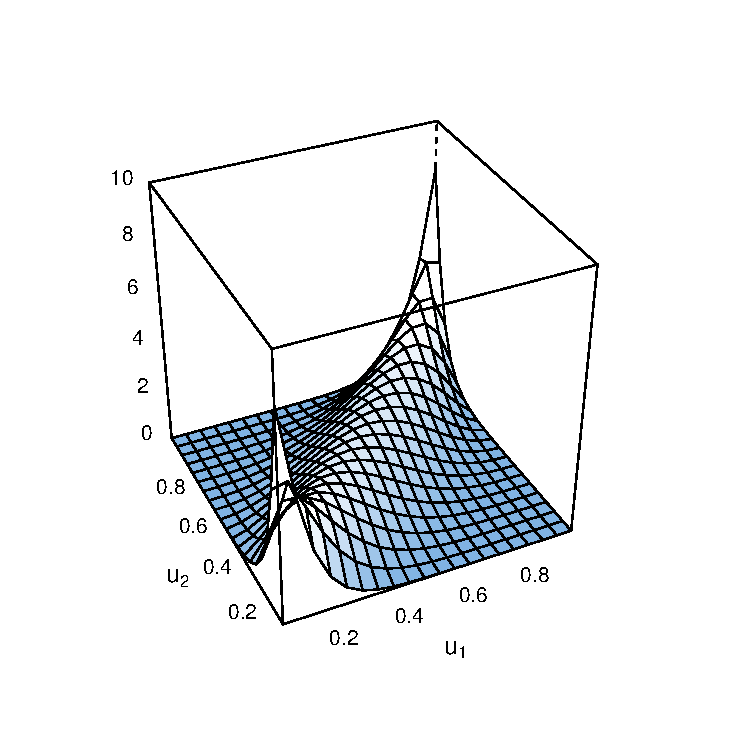
\includegraphics[trim= 1cm 1cm 2cm 1cm, clip=true, width = .5\textwidth]{Figures/Fig-1-1/gaussian-copula.pdf}
	}
	\hfill
	\subfloat{%
		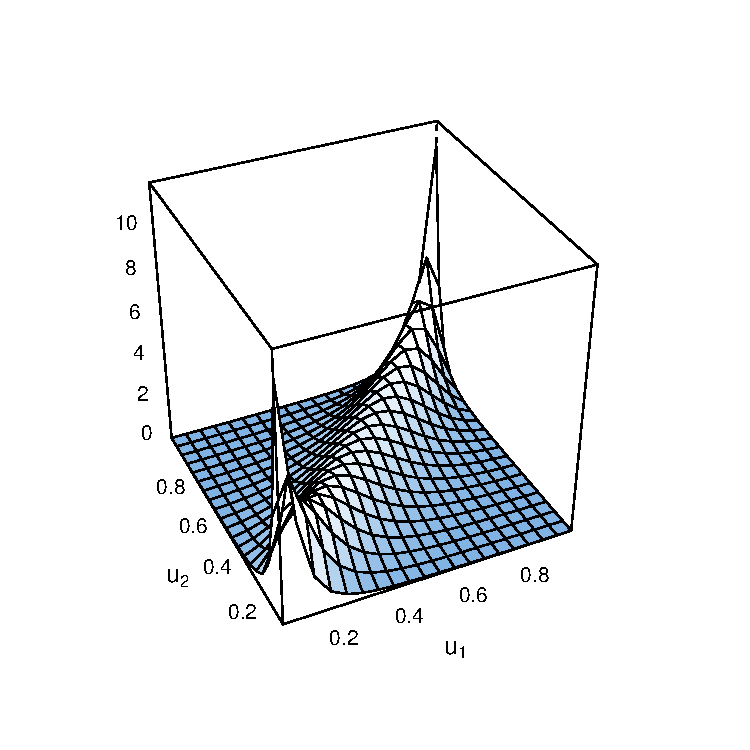
\includegraphics[trim= 1cm 1cm 2cm 1cm, clip=true, width = .5\textwidth]{Figures/Fig-1-1/t-copula.pdf}
	}
	\hfill
	\subfloat{%
		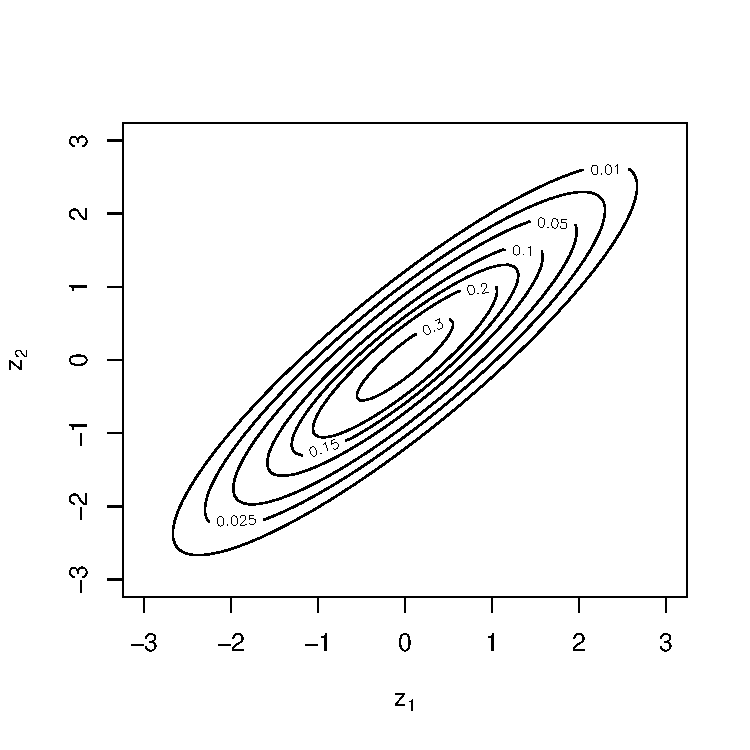
\includegraphics[trim= 0cm 0cm 0cm 2cm, clip=true, width = .5\textwidth]{Figures/Fig-1-1/gauss-contour.pdf}
	}
	\hfill
	\subfloat{%
		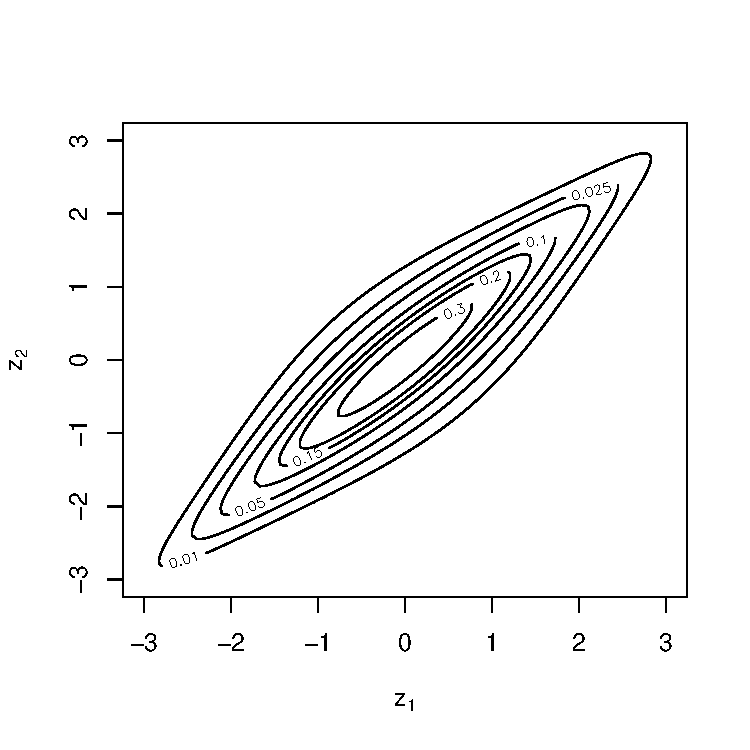
\includegraphics[trim= 0cm 0cm 0cm 2cm, clip=true, width = .5\textwidth]{Figures/Fig-1-1/t-contour.pdf}
	}
	\caption[\textsc{Bivariate elliptical copula densities:} A comparison between Gaussian and $t$-copulae]{\textsc{Bivariate elliptical copula densities:} Top: three-dimensional density plots of a theoretical Gaussian copula (left) and a $t$-copula with $\nu = 4$ degrees of freedom (right). The parameters have been chosen in such a way that Kendall's $\tau = 0.7$. Below are the respective contour plots belonging to the densities. The plots were generated using the BiCop function from the VineCopula package in R.}
	\label{dens-cont-normal-t}
\end{figure}

\subsection{Archimedean copulae}

Archimedean copulae and their detailed properties have already been discussed by for example \citet{nelsen2007introduction} or \citet{mcneil2009multivariate}. Therefore, we now derive just the fundamental building blocks for bivariate Archimedean copulae.

Following the work of \citet{genest1993statistical} a copula is called \textit{Archimedean} if it can be expressed as

\begin{equation}
	C_{\varphi}\left( \mathbf{u}\right) = \varphi ^{[-1]}\left( \varphi \left( u_1\right) +\dots +\varphi \left( u_d\right) \right),
\end{equation}
%
for some continuous, strictly monotone decreasing, and convex function $\varphi : \mathbf{I} \rightarrow \left[ 0,\infty \right] $, satisfying $\varphi \left( 1 \right)=0$ and $\mathbf{I}$ being the unit interval. This function is called the \textit{generator function} for the copula and is furthermore called \textit{strict} if $\varphi \left( 0 \right) = \infty$. $\varphi ^{[-1]}$ is the pseudo-inverse satisfying the following conditions

\begin{equation}
	\varphi^{[-1]}(t):=\left\{\begin{array}{ll}
		\varphi^{-1}(t)&, 0 \leq t \leq \varphi(0) \\
		0 & , \varphi(0) \leq t \leq \infty .
	\end{array}\right.
\end{equation}

We will now present the Archimedean copulae with its generators and properties that this simulation study will use. To date there has been defined a wide variety of Archimedean copulae with contrasting properties (see \citet{nelsen2007introduction} for a comprehensive list).

For $\varphi_\theta \left( u\right) = \left(- \log\left(u \right)\right)^{\theta} $ with $\theta \in \left[ 1,\infty\right) $ we attain the Gumbel copula. We include it in this simulation because it is representative for the subclass of asymmetric tail dependent copulae (upper tail dependence only) while the Gaussian and $t$-copulae represent either tail independence or symmetric tail dependence respectively. We will formally introduce this property in the next section. The Gumbel distribution function is defined as

\begin{equation}
	C_{\theta}^{G}\left(\mathbf{u}; \theta\right)=\exp \left[-\left\{\sum_{j=1}^{d}\left(\log u_{j}\right)^{\theta}\right\}^{\frac{1}{\theta}}\right] .
\end{equation}

Just like the Gaussian copula from the elliptical class there exists an Archimedean one that is symmetrically tail independent, the Frank copula. The generator is defined by $\varphi_{\theta}(u)=-\log \left\{\frac{\exp (-\theta u)-1}{\exp (-\theta)-1}\right\}$ with $\theta \in \left(-\infty, \infty \right) \setminus \left\lbrace 0\right\rbrace$. The accompanying cdf can now easily be derived as

\begin{equation}
	C_{\theta}^{F}\left( \mathbf{u}; \theta \right)=-\frac{1}{\theta} \log \left[1+\frac{\prod_{j=1}^{d}\left\{\exp \left(-\theta u_{j}\right)-1\right\}}{\{\exp (-\theta)-1\}^{d-1}}\right] .
\end{equation}  

The last copula that we will include in the simulation is the Clayton copula, named after its discoverer in \citet{clayton1978model}. It somewhat resembles the counterpart to the Gumbel copula as it is only lower tail dependent. Its generator is defined by $\varphi_{\theta}(u)=\frac{1}{\theta}\left(u^{-\theta}-1\right)$ for $\theta \in\left[-\frac{1}{d-1}, \infty\right) \backslash\{0\}$, which lets us define its distribution as 

\begin{equation}
	C_{\theta}^{Cl}\left(\mathbf{u}; \theta\right)=\left\{\left(\sum_{j=1}^{d} u_{j}^{-\theta}\right)-d+1\right\}^{-\frac{1}{\theta}}
\end{equation}

To get a graphical intuition about the different presented copulae, their three-dimensional bivariate densities and the respective contour plots are given in Figure \ref{dens-cont-arch}.

\begin{figure}[!ht]
	\subfloat{%
		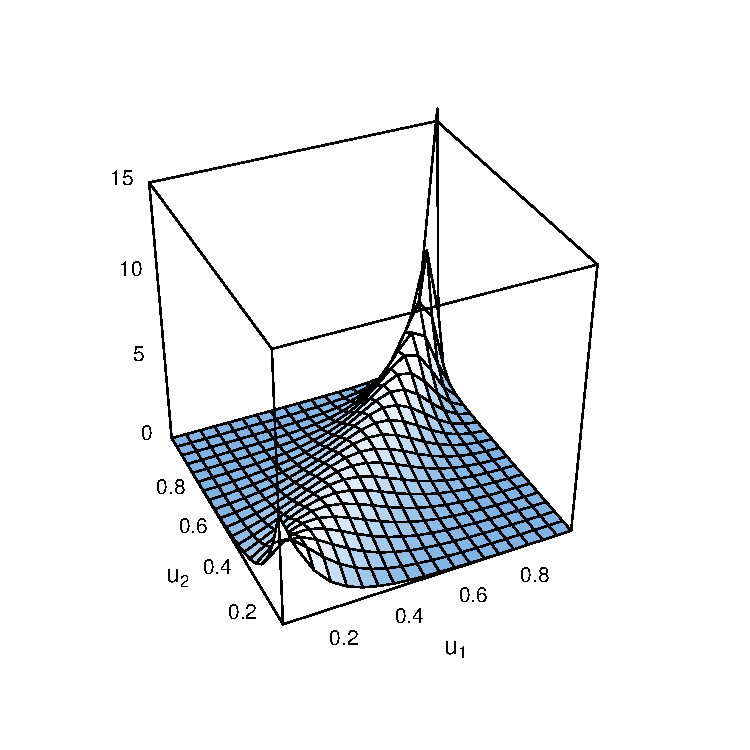
\includegraphics[trim= 1.8cm 1cm 2cm 1cm, clip=true, width = .32\textwidth]{Figures/Fig-1-2/gumbel-dens.pdf}
	}
	\hfill
	\subfloat{%
		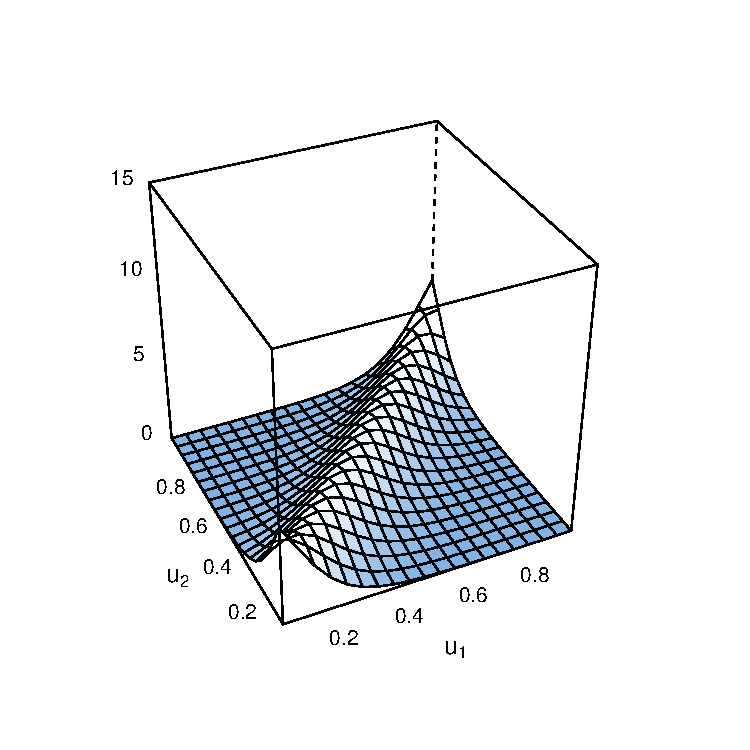
\includegraphics[trim= 1.8cm 1cm 2cm 1cm, clip=true, width = .32\textwidth]{Figures/Fig-1-2/frank-dens.pdf}
	}
	\hfill
	\subfloat{%
		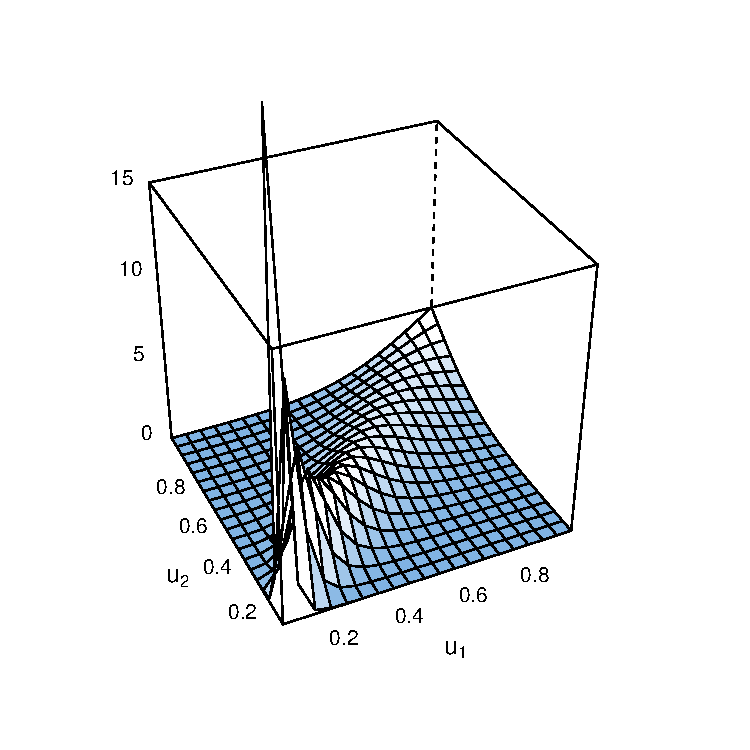
\includegraphics[trim= 1.8cm 1cm 2cm 1cm, clip=true, width = .32\textwidth]{Figures/Fig-1-2/clayton-dens.pdf}
	}
	\hfill
	\subfloat{%
		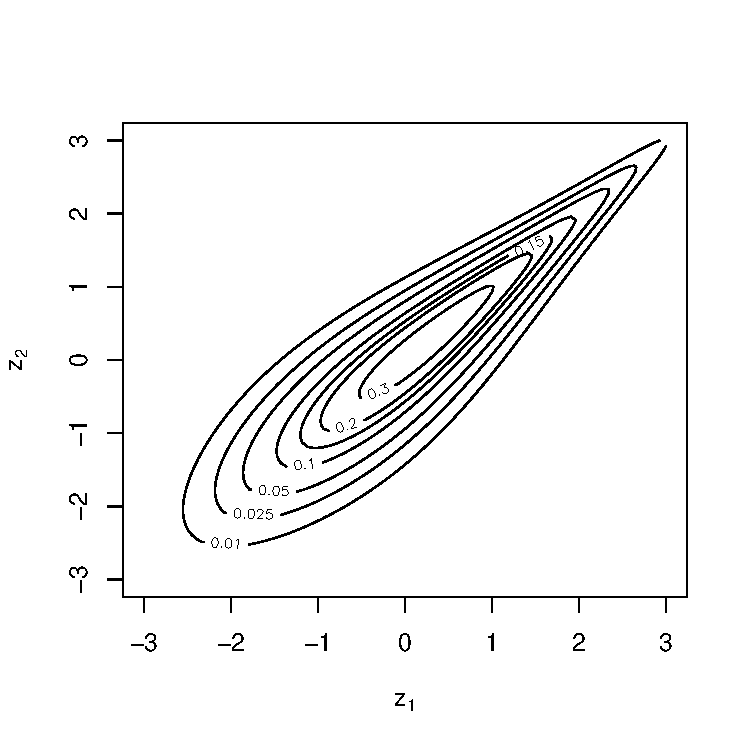
\includegraphics[trim= 0cm 0cm 0cm 2cm, clip=true, width = .32\textwidth]{Figures/Fig-1-2/gumbel-contour.pdf}
	}
	\hfill
	\subfloat{%
		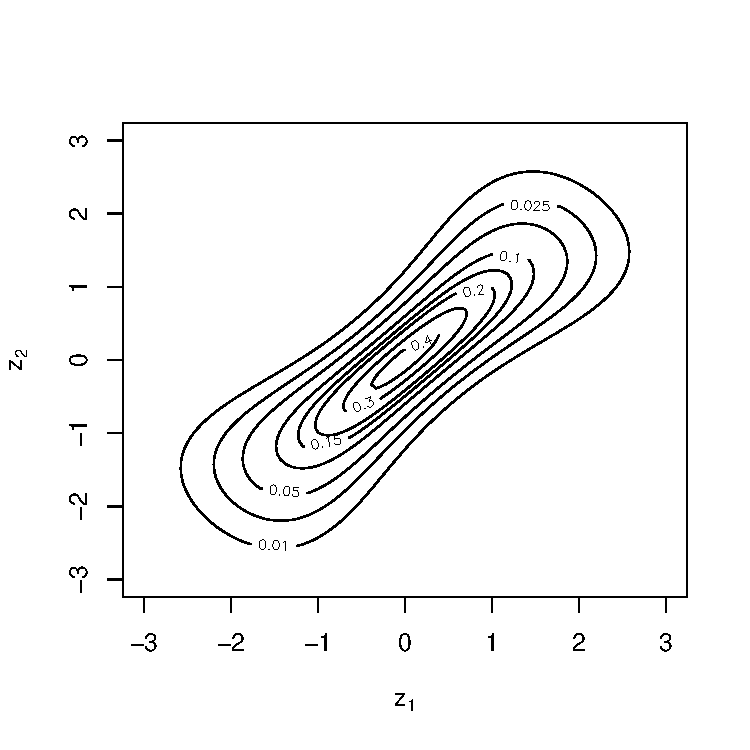
\includegraphics[trim= 0cm 0cm 0cm 2cm, clip=true, width = .32\textwidth]{Figures/Fig-1-2/frank-contour.pdf}
	}
	\hfill
	\subfloat{%
		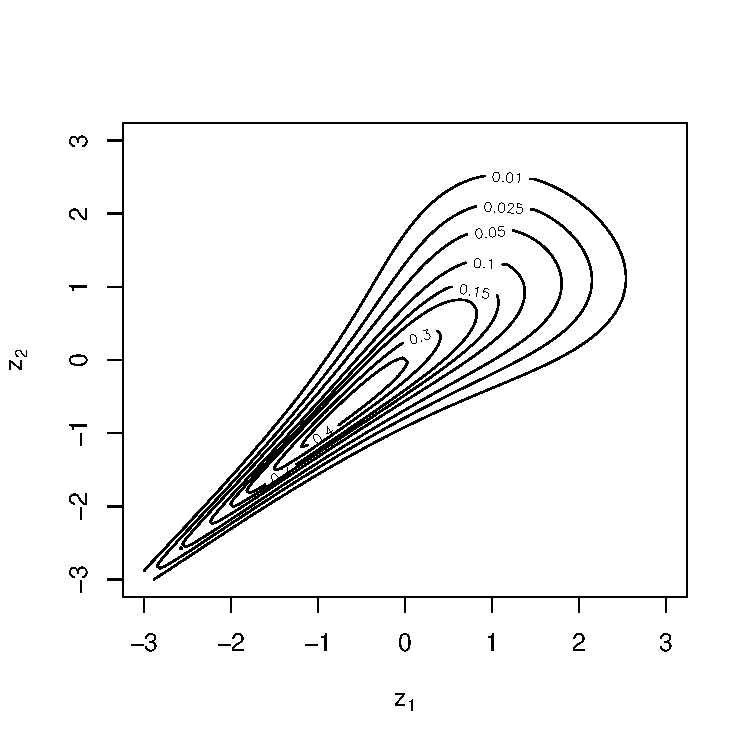
\includegraphics[trim= 0cm 0cm 0cm 2cm, clip=true, width = .32\textwidth]{Figures/Fig-1-2/clayton-contour.pdf}
}
	\caption[\textsc{Bivariate Archimedean copula densities:} A comparison between Gumbel, Frank and Clayton copulae]{\textsc{Bivariate Archimedean copula densities:} Top: three-dimensional density plots for theoretical Gumbel (left), Frank (middle) and Clayton (right) copulae. The parameters have been chosen in such a way that Kendall's $\tau = 0.7$. Below are the respective contour plots belonging to the densities.}
	\label{dens-cont-arch}
\end{figure}


\section{Dependence measures}

We will now, first, introduce the concept of the aforementioned tail dependence and, second, describe two ways to quantify the existence, direction and strength of dependence between two random variables and their connection to the dependence structure of a copula. The first of which will be \textit{Kendall's Tau} and the second \textit{Blomqvist's Beta}. There also exists a variety of other dependence measures; for the sake of simplicity, however, we will only present those needed for our simulation study. 

\subsubsection*{Tail dependence}

The concept of tail dependence arises from extreme value theory and quantifies the joint presence of either very small or very large values or both via a tail-dependence-coefficient. Given two random variables $X_1$ and $X_2$ it is defined by the limit

\begin{equation}
	\lambda^{\mathrm{u}}=\lim _{q \rightarrow 1^{-}} P\left(X_{2}>F_{2}^{-1}(q) \mid X_{1}>F_{1}^{-1}(q)\right)=\lim _{q \rightarrow 1^{-}} \frac{1-2 q+C(q, q)}{1-q} 
\end{equation}
%
for upper tail dependence and

\begin{equation}
	\lambda^{\mathrm{l}}=\lim _{q \rightarrow 0^{+}} P\left(X_{2} \leq F_{2}^{-1}(q) \mid X_{1} \leq F_{1}^{-1}(q)\right)=\lim _{q \rightarrow 0^{+}} \frac{C(q, q)}{q}
\end{equation}
%
for lower tail dependence. The coefficient's support is on $0 \leq \lambda^{\mathrm{u}},\lambda^{\mathrm{l}} \leq 1 $ and can be understood as a measure of strength, getting closer to one, the closer the link between X reaching large values and Y reaching large values likewise. A more detailed introduction into extreme value theory can be found in Chapter 7 of \citet{mcneil2015quantitative}.

\subsubsection*{Kendall's Tau}

\textit{Kendall's Tau} \citep*{kendall1938new} is a rank based correlation coefficient that splits the present data into concordant or discordant pairs and calculates its difference. Suppose there is a set of $x$-sorted observations $\left(x_i , y_i \right)$ for $ i \in \left\lbrace 1,\dots ,n \right\rbrace $ and $x_1 <x_2 < \dots < x_n$, then two pairs of variables $\left( x_i , y_i \right) $ and $\left( x_j , y_j \right)$ for $i<j$ are called \textit{concordant} if either both $x_i > x_j$ and $y_i > y_j$ or $x_i < x_j$ and $y_i < y_j$, otherwise they are called \textit{discordant}.

The product of their differences is summed up and divided by $ {n\choose 2} = \frac{n(n-1)}{2}$ to build the empirical $\tau$-coefficient defined as

\begin{equation}
	\label{emp-kendall}
		\hat{\tau}:=\frac{2}{n(n-1)} \sum_{i<j} \mathrm{sgn}\left(x_{i}-x_{j}\right) \mathrm{sgn}\left(y_{i}-y_{j}\right)
\end{equation}
%
with $ \mathrm{sgn}\left(\cdot \right) $ being the signum function. $\hat{\tau}$ can take any value in $\left[ -1,1 \right] $ where $-1$ and $+1$ imply perfect negative or positive dependence respectively. The provided formula above does not allow for ties where $\mathrm{sgn}\left(x_{i}-x_{j}\right) \mathrm{sgn}\left(y_{i}-y_{j}\right) = 0$. Kendall's Tau is directly connected to the bivariate copula distribution via (see Appendix \ref{AppendixA} for proof)

\begin{equation}
	\label{tau-copula}
		\tau=-1+4 \int_{[0,1]^{2}} C\left(u_{1}, u_{2}\right) \mathrm{d} C\left(u_{1}, u_{2}\right) .
\end{equation}

The fact that Kendall's Tau is solely dependent on the copula allows us to estimate the copula parameter $\theta$ via the inverse of \ref{tau-copula} such that $\tau (C_\theta) = \hat{\tau}$. This will be discussed in more detail when we introduce the copula estimators for our simulation in Chapter 2.

\subsubsection*{Blomqvist's Beta}

An even simpler way to measure bivariate dependence is the use of \textit{Blomqvist's Beta}, first described by \citet{blomqvist1950measure}. The idea is to divide the data plane into four quadrants and count all respective observations via a $2 \times 2$ contingency matrix. From this Blomqvist's $\beta$ is constructed as follows:

Let $\tilde{X}$ and $\tilde{Y}$ be the respective medians of two random variables $X_1, \dots , X_n$ and $Y_1, \dots , Y_n$. To construct a useful measure of dependence, the $x-y$ plane is then divided into four parts by splitting it at $x=\bar{X}$ and $y=\bar{Y}$ and counting all points that lie in diagonally opposing quadrants. We then define $n_1$ as the number of points in the lower left and upper right region and $n_2$  as the number of points in the upper left and lower right region to construct the empirical Blomqvist's Beta

\begin{equation}
	\hat{\beta}=\frac{n_{1}-n_{2}}{n_{1}+n_{2}}=\frac{2 n_{1}}{n_{1}+n_{2}}-1 ,
\end{equation}
%
where $-1\leq \hat{\beta} \leq 1$. For an odd sample size, either one or two points must lie on one or both segmenting lines $x=\tilde{X}$ and $y=\tilde{Y}$ respectively, which raises the question to which quadrant the point will be counted. Blomqvist suggests that for one point lying on a median line, it shall be ignored, while in the case of two points lying on both segmenting lines, one is ignored and the second is counted to the quadrant both points adjoin.

From the population analogue of Blomqvist's Beta 

\begin{equation}
	\beta=P\{(X-\tilde{X})(Y-\tilde{Y})>0\}-P\{(X-\tilde{X})(Y-\tilde{Y})<0\} ,
\end{equation}
%
one can derive the Copula representation (done in Appendix \ref{AppendixA}) which is given by

\begin{equation}
	\label{beta-copula}
	\beta=4 C\left( F_{X}(\tilde{X}), F_{Y}(\tilde{Y})\right) -1 =4 C\left(\frac{1}{2}, \frac{1}{2}\right) -1
\end{equation}
%
This representation allows us estimate the copula parameter $\theta$ by solving the equation $\beta (C_\theta)=\hat{\beta}$. For both inversion methods it is assumed that $C \in C_\theta$ and $\theta \in \mathbb{R}$.

\chapter{Copula selection and parameter estimation} 

\label{Chapter2}

%----------------------------------------------------------------------------------------
%	SECTION 1
%----------------------------------------------------------------------------------------

\section{Estimation methods}
\label{est-methods}

The simulation in this article uses three different estimators to select and parameterize bivariate copulae. The first one will be the classical maximum likelihood estimator, while the last  two are the inverses of the just presented moment-based functions, Kendall's Tau and Blomqvist's Beta. A similar study just for the parameter estimation process has already been done by \citet{genest2013copula}, finding that the ML-estimator is the most precise in every application, yet it is slower. This is congruent to other studies comparing maximum likelihood to several other estimators, for example \citet{weiss2011copula}.

The following section details how the just presented estimators operate and how the estimation process will take place. In a first step I will present how the parameter describing a copula distribution is estimated given that the true copula is known, and in a second step I will use a selection criterion in combination with the parameter to select the best copula out of a range. For this step I suppose that the true copula is not known.

\subsection{Maximum likelihood}

At the beginning of a bivariate estimation process one needs to specify the marginal distributions of the available data. Suppose an i.i.d sample of bivariate data $\left\lbrace x_{i1},x_{i2}\right\rbrace$ for $i = 1,\dots , n$. If the marginal distribution is known the copula data can be directly obtained using the probability integral transform

\begin{equation}
	\label{known-margins}
	\left(u_{i 1}, u_{i 2}\right):=\left(F_{1}\left(x_{i 1}\right), F_{2}\left(x_{i 2}\right)\right) \text {\qquad for } i=1, \ldots, n .
\end{equation}

In real-world data applications, however, margins are rarely known, so \citet{oakes1994multivariate} suggested replacing them with their empirical versions

\begin{equation}
	\label{emp-margins}
	\hat{F_j}(x_j)=\frac{1}{n+1} \sum_{i=1}^{n} \mathbf{1}_{\left(x_{ij} \leq x_j\right)} \text{\qquad for } j = \left\lbrace 1,2 \right\rbrace ,
\end{equation}
%
with $\mathbf{1}_{(E)}$ being the indicator function for event $E$. To avoid boundary problems in further calculations as $\hat{F}(x_{nj}) \approx 1$, it is convenient to use the re-scaled version of \citet{genest1995semiparametric} which you see in the equation above. Here, the factor $\frac{1}{n+1}$ replaces the problematic $\frac{1}{n}$ in the old version.

The generated observations using the empirical margins are called \textit{pseudo observations} and for $n \rightarrow \infty$ the empirical margin estimator converges towards the real marginal distribution. However, even if misspecified marginal distributions are used, the overall effect on model validity is insignificant as long as the margin of error does not grow too large \citep{kim2007comparison}.

To estimate parameters via maximum likelihood we require the copula to be an element of all parameterized copulae $C \in (C_\theta)$ and the parameter $\theta$ to be real valued. If the copula for the observations $\left\lbrace x_{i1},x_{i2}\right\rbrace$ has a density for all $u_1,u_2 \in (0,1)$ given by 

\begin{equation*}
	c_{\theta}(u_1, u_2)=\frac{\partial^{2}}{\partial u_1 \partial u_2} C_{\theta}(u_1, u_2),
\end{equation*}
%
the log-likelihood function for $\theta$, given known margins is defined as

\begin{equation}
	\ell(\theta)=\sum_{i=1}^{n} \log \left[c_{\theta}\left\{F_1\left(x_{i1}\right), F_2\left(x_{i2}\right)\right\}\right].
\end{equation}

In the more practical case of unknown margins, they are, as mentioned above, replaced by their empirical versions to yield 

\begin{equation}
	\ell(\theta)=\sum_{i=1}^{n} \log \left[c_{\theta}\left\{\hat{F}_1\left(x_{i1}\right), \hat{F}_2\left(x_{i2}\right)\right\}\right],
\end{equation}
%
where

\begin{equation}
	\label{ml-estimation}
	\hat{\theta}_{n}^{M L}(u_1,u_2) \equiv \underset{\theta \in \Theta}{\arg \max } \ell (\theta).
\end{equation}

As \citet{genest1995semiparametric} showed, the maximum likelihood estimator is consistent and asymptotically normal under regularity conditions.

\subsection{Inverse of Kendall's Tau}

Following equation \ref{tau-copula} there is a direct connection between the copula distribution and the Kendall rank correlation coefficient. For the inversion method we choose a copula family that has an explicit relationship between its parameter $\theta$ (or $\rho$ for elliptical copulae) and Kendall's $\tau$ such that

\begin{equation*}
	\tau = \delta (\theta), 
\end{equation*}
%
with $\delta (\cdot)$ being the respective copula-tau relationship function calculated from \ref{tau-copula}. From this we can directly derive an estimator for $\theta$ by inverting the relationship function and using the empirical version of $\tau$ as its argument, yielding

\begin{equation}
	\hat{\theta}_\tau := \delta^{-1}(\hat{\tau}). 
\end{equation}

For the copulae introduced in Chapter \ref{Chapter1} the relationship function and their inverses can be found in Table \ref{iTau-rel-funcs}.

\begin{table}
	
	\centering
{\renewcommand{\arraystretch}{1.4}
\begin{tabular}{c|l|l}
	\hline
	Copula family & $\delta(\theta)$ or $\delta(\rho)$ & $\delta^{-1}(\hat{\tau})$ \\
	\hline
	\hline
	Gaussian & $\tau=\frac{2}{\pi} \arcsin (\rho)$ & $\hat{\theta}_\tau =\sin(\hat{\tau}\frac{\pi}{2})$ \\
	\hline
	Students \textit{t}& $\tau=\frac{2}{\pi} \arcsin (\rho)$ & $\hat{\theta}_\tau =\sin(\hat{\tau}\frac{\pi}{2})$ \\
	\hline
	Clayton & $\tau = \frac{\theta}{\theta + 2}$ & $\hat{\theta}_\tau =2\frac{\hat{\tau}}{1-\hat{\tau}}$ \\
	\hline
	Gumbel & $\tau = 1-\frac{1}{\theta}$ & $\hat{\theta}_\tau =\frac{1}{1-\hat{\tau}}$ \\
	\hline
	Frank & $\tau = 1- \frac{4}{\theta}+4\frac{D_1(\theta)}{\theta}$ with & no closed  \\
	& $D_{1}(\theta)=\int_{0}^{\theta} \frac{x / \theta}{e^{x}-1} d x$ & form expression \\
\end{tabular}
}
	\caption[Relationship functions and inverses for the inversion of Kendall's Tau]{Relationship functions for selected copulae and their inverses. For the Gaussian and t-copula, the dependence parameter is called $\rho$ and will, therefore be the argument of its function.}
	\label{iTau-rel-funcs}
\end{table}

\subsection{Inverse of Blomqvist's Beta}

As with the inversion of Kendall's Tau there also exists a direct connection between the copula parameter $\theta$ or $\rho$ and Blomqvist's Beta via equation \ref{beta-copula}. The major difference between $\beta$-inversion and $\tau$-inversion is the algorithmic complexity. While the first has a linear complexity of $\mathcal{O}(n)$, the latter has quadratic complexity $\mathcal{O}(n^2)$ (\cite[see][]{genest2013copula}) and is thus computationally more challenging.

To derive an estimator for Blomqvist's Beta, the same process is used as for the inversion of Kendall's Tau. At first, a one to one relation of the form 

\begin{equation*}
	\beta = \varrho (\theta), 
\end{equation*}
%
is used to then find an inverse that acts as an estimator for the copula parameter given an estimate of Blomqvist's Beta

\begin{equation}
	\hat{\theta}_\beta := \varrho^{-1}(\hat{\beta}). 
\end{equation}

As above I will provide a table with all relationship functions and their respective inverses used in this simulation study i.e. Table \ref{iBeta-rel-funcs}. Notice that for the Gumbel estimator $\hat{\theta}_\beta$ there is no analytic inverse for the complete range of $\hat{\beta} \in\left[-1,1 \right] $ so I use a pseudo-inverse which is only well defined for $\hat{\beta} \in\left[0,1 \right)$. For the implementation of this simulation the pseudo-inverse can be used without problems as only positive dependencies and, thus, parameters are estimated. The inverse relationship functions which do not have closed form expressions will be inverted numerically.
\begin{table}

	\centering
	{\renewcommand{\arraystretch}{1.4}
		\begin{tabular}{c|l|l}
			\hline
			Copula family & $\varrho (\theta)$ or $\varrho (\rho)$ & $\varrho^{-1}(\hat{\beta})$ \\
			\hline
			\hline
			Gaussian & $\beta=\frac{2}{\pi} \arcsin (\rho)$ & $\hat{\theta}_\beta =\sin(\hat{\beta}\frac{\pi}{2})$ \\
			\hline
			Students \textit{t}& $\beta=\frac{2}{\pi} \arcsin (\rho)$ & $\hat{\theta}_\beta =\sin(\hat{\beta}\frac{\pi}{2})$ \\
			\hline
			Clayton & $\beta = -1+4(2^{\theta +1}-1)^{-1 / \theta}$  & no closed \\
			& & form expression\\
			\hline
			Gumbel & $\beta = -1+4\exp\left[ -\log(2) \cdot 2^{1/\theta} \right] $ &  $\hat{\theta}_\beta = -\frac{\log (2)}{\log \left(-\frac{\log (2)}{\log \left(\frac{\hat{\beta}+1}{4}\right)}\right)}$ \\
			& & only for $\hat{\beta} \in \left[ 0,1 \right) $ \\
			\hline
			Frank & $\beta = \frac{4}{\theta}\log\cosh \frac{\theta}{4}$ & no closed  \\
			& & form expression \\
		\end{tabular}
	}
	\caption[Relationship functions and inverses for the inversion of Blomqvist's Beta]{Relationship functions for selected copulae and their inverses for the inversion of Blomqvist's Beta. For the Gaussian and t-copula, the dependence parameter is called $\rho$ and will, therefore be the argument of its function.}
	\label{iBeta-rel-funcs}
\end{table}


\section{Copula selection strategy}

So far I described the process of finding a suitable parameter for known data and a known copula. In real-world applications, however, the underlying or true copula is rarely, if ever, known so one needs a process that selects an appropriate copula from a given set of data $\left\lbrace x_{i1},x_{i2}\right\rbrace$ for $i = 1,\dots , n$. 

In a first step the data needs to be transformed to the copula scale $u_{i1},u_{i2}\in \left[ 0,1 \right] $ via the probability integral transform. This can be done either via equation \ref{known-margins} for known margins or via equation \ref{emp-margins} for unknowns. In my simulation this step is skipped as I will derive the observations directly from a copula. 

In the next step, the transformed data is fitted to every available copula as described in section \ref{est-methods}. This yields one parameter per copula per estimator. To now find the model with the best fit based upon the estimates, I use the Akaike Information Criterion (AIC) \citep{akaike1973information} defined as:

\begin{equation}
	\label{AIC}
	AIC:=-2 \sum_{i=1}^{n} \log \left[c\left(u_{i1}, u_{i2} \mid \hat{\boldsymbol{\theta}}\right)\right]+2p,
\end{equation}
%
with $p$ being the number of parameters; for this study $p = 1$ as only one-parameter copulae are estimated.

Since both inversion methods do not depend on likelihood functions when estimating parameters, the AIC as a comparing selection criterion can only be used by plugging the inversion-estimates back into the log-likelihood function found for the maximum likelihood procedure. Thus, an AIC for every estimator can be obtained by setting:

\begin{equation}
	\label{estimators}
	\hat{\boldsymbol{\theta}} := \left\{\begin{array}{lll}
			\hat{\theta}_{n}^{ML} &, \text{for ML} \\
			\delta^{-1}(\hat{\tau}) &, \text{for Kendall's Tau inversion}\\
			\varrho^{-1}(\hat{\beta}) &, \text{for Blomqvist's Beta inversion}.
	\end{array}\right.
\end{equation}

In a last step the copula with the smallest AIC value per estimator is selected. By means of the AIC, the so chosen model is the most parsimonious. 

In this simulation I will record the relative computation time it takes for every estimator to select a copula from the data on the basis of AIC. I expect the inversion methods to be significantly faster than ML as they skip the optimization process (equation \ref{ml-estimation}) for ML, which is computationally challenging, especially with large sample sizes. 

\chapter{Simulation study} 

\label{simulation-study}

A sizable Monte-Carlo simulation study has been carried out to test the performance, accuracy and computational efficiency of the three presented estimators (maximum likelihood, Kendall's Tau inversion and Blomqvist's Beta inversion) in terms of copulae parameter estimation and selecting an appropriate copula from data. To measure parameter-estimation-accuracy, the mean-square-error (MSE) for every parameter estimate per estimator is calculated and averaged over a large number of experiments. The performance is determined via relative computation time it takes for my algorithm to converge. I do not use absolute values, because they carry no additional information about computational performance but much rather about the specific hardware I am using.

In terms of selecting one copula for a given set of data, relative computation time for my algorithm to converge to one copula is measured per estimator. The validity of its choice is also denoted.

\section{Procedure}

The design of this simulation study will base on several other studies that measure performance of different parameter estimators for copulae in a Monte-Carlo manner such as \citet{kim2007comparison}, \citet{kojadinovic2010comparison}, \citet{weiss2011copula} or \citet{genest2013copula}.

For every parametric copula presented above the following steps are repeated $k$ times in sequence fr the parameter estimation:

\begin{enumerate}
	\itemsep0em
	\item A sample of size $n$ is simulated from a theoretical copula $C \in (C_\theta)$ with true parameter $\theta$.
	\item Compute the parameter estimates with the maximum-likelihood and each of the moment-based inverses under the premise that the parametric form of the copula is known.
	\item Calculate the average MSE per parameter by $MSE(\hat{\boldsymbol{\theta}}) \equiv k^{-1}   \sum_{i=1}^{k} E\left[ \theta - \hat{\boldsymbol{\theta}}_i \right]^2 $, with $\theta$ being the true parameter and $\hat{\boldsymbol{\theta}}$ being the estimated parameter vector from equation \ref{estimators} for every iteration.
	\item Provide relative computation time per estimator per copula, where median maximum-likelihood time is set to 100 ($\tilde{t}_{ML} = 100$). All benchmarking exercises are done using the \verb*|microbenchmark| package.
\end{enumerate}

For this study I will set $k = 1000$ and $ n = \left\lbrace 30,50,100 \right\rbrace $ similar to other studies provided above. The optimization process for maximum-likelihood uses a bounded, limited-memory BFGS algorithm, which has been proven to be an optimal choice for maximum entropy problems \citep{malouf2002comparison}. I will test the whole process for a range of parameter values. For the elliptical copulae I use $\rho \in \left\lbrace -0.9,-0.8 \dots 0.8,0.9 \right\rbrace $ while for the archimedean copulae I use $\theta \in \left\lbrace 1,1.5 \dots 9.5,10 \right\rbrace $. I will set the degrees of freedom for the $t$-copula fix to $\nu = 4$ as it drastically increases computational speed since the estimation process for the degrees of freedom can be circumvented \citep{lucas2014conditional}. 

The copula selection process will follow a similar fashion as the parameter estimation. The following process is repeated $k$ times:

\begin{enumerate}
	\itemsep0em
	\item A sample of size n is simulated from a known copula $C \in (C_\theta)$ with known parameter $\theta$.
	\item The sample is fitted to every copula available for each estimator and respective AIC values are computed.
	\item Copula with lowest AIC per estimator is chosen. Correct selections over $k$ are returned ($\frac{\# \text{of correct selections}}{k}$).
	\item Relative computation times per copula and estimator are computed. Again done with the \verb*|microbenchmark| package.
\end{enumerate}

During the copula selection procedure, I use $k = 100$ and  $ n = \left\lbrace 30,100 \right\rbrace $. As with the parameter estimation, the range of parameters per copula and estimator will remain the same.

The simulation is performed on version \verb*|4.0.3| of \verb*|R|. The copula observations are simulated using the \verb*|BiCopSim| function from the \verb*|VineCopula| package.

\section{Results}

The results of the parameter estimation study are shown in Figures \ref{gauss_t_sim}, \ref{clayton-gumbel-sim} and \ref{frank-sim}. Relative computation time can be found in table \ref{rel-comp-time-est}. The figures show the average mean-square-error for every estimator and parameter for $1000$ repetitions per parameter step. The sample size $n = 50$ is omitted in the figures as the result is congruent with the evidence showing that accuracy increases with sample size for all estimators.

\subsection{Estimator choice for parameter estimation}

Interestingly, the results show a relatively uniform behavior for the inversion of Kendall's Tau and maximum likelihood estimators. Regardless of the magnitude of dependence, both estimators show very small MSEs across all parameters with Tau's inversion being slightly inferior in high dependence scenarios for archimedean copula where $\theta > 6$. 

The relative computation times from Table \ref{rel-comp-time-est} reveal that, although being approximately equally accurate, Kendall's Tau inversion can be more than ten times faster than maximum likelihood. This outcome occurs when the density functions of the respective copulae are computationally challenging as for example with the $t$-copula. Vice versa, in scenarios where there is no closed form relationship function between the copula and its dependence measure, computation time is almost equal, i.e Tau inversion for the Frank copula still needs $92.3\%$ of the time it takes ML to converge.

Blomqvist's Beta inversion is not recommended to use for parameter estimation under any circumstance. It may be faster to compute in some situations, however, the large margin of error can make predictions error-prone and unpredictable. This is especially evident in extreme value copulae such as the Gumbel copula, with MSE values exceeding ten.

\begin{figure}[!ht]
	\subfloat{%
		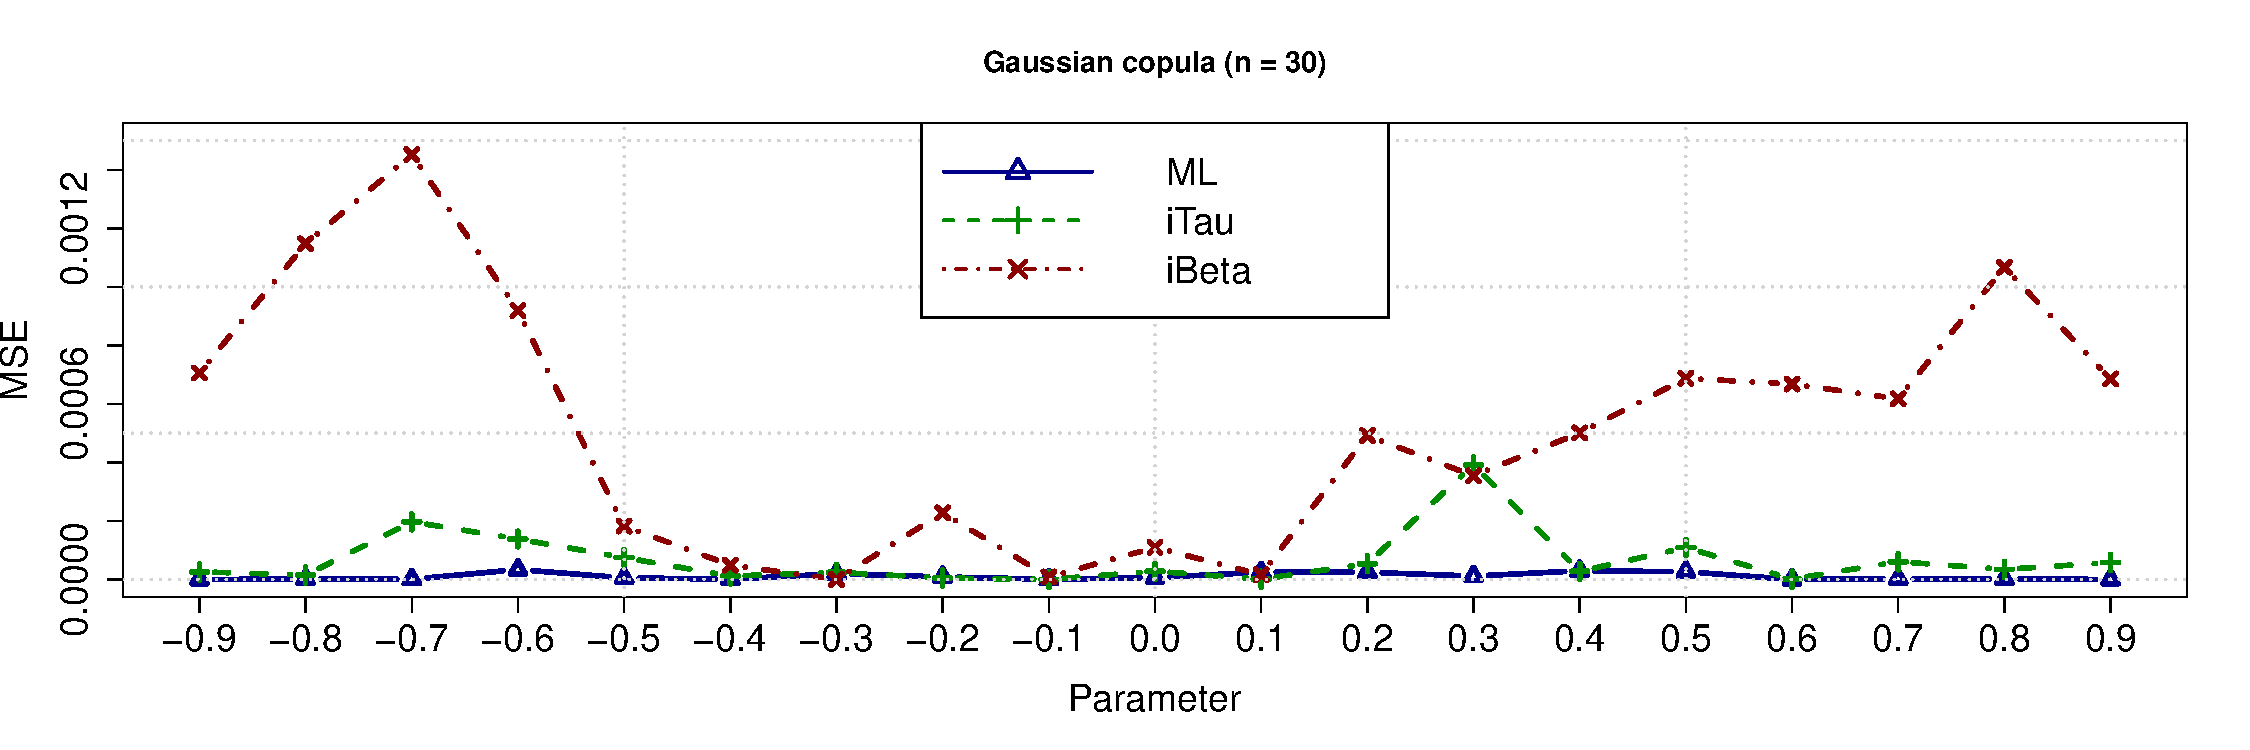
\includegraphics[trim= 0cm 1.6cm 1cm 0cm, width = .98\textwidth]{Figures/mc-plots/gaussian30.pdf}
	}
	\hfill
	\subfloat{%
		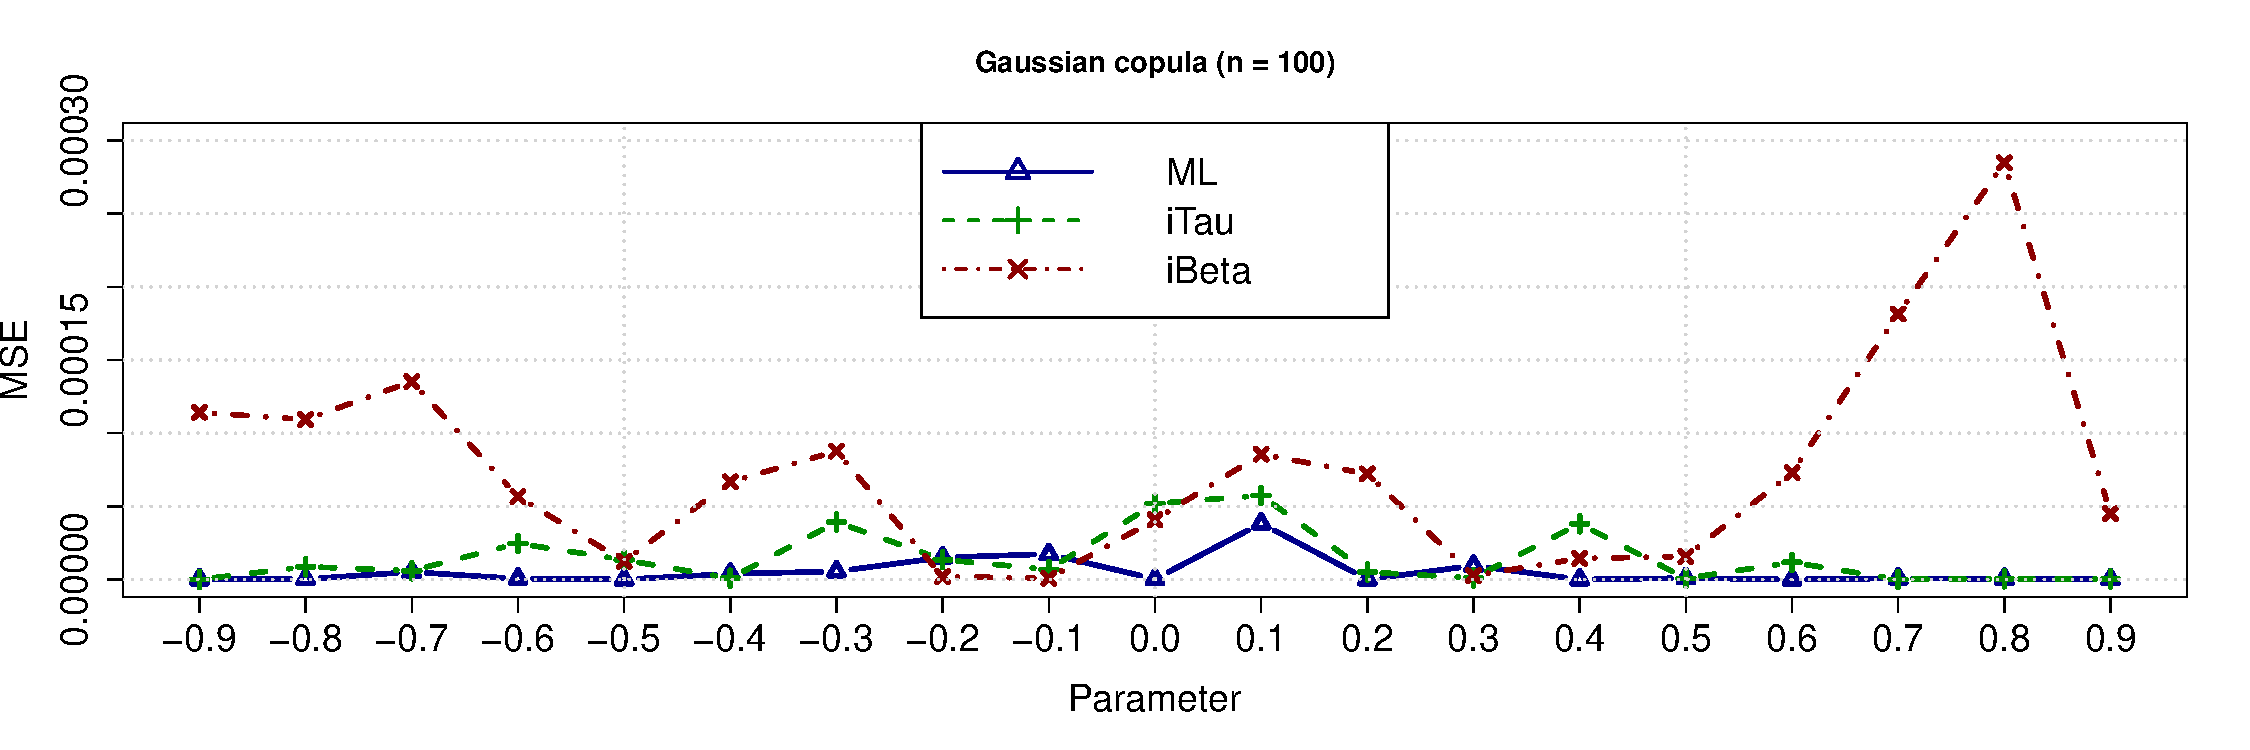
\includegraphics[trim= 0cm 1.6cm 1cm 0cm,width = .98\textwidth]{Figures/mc-plots/gaussian100.pdf}
	}
	\hfill
	\subfloat{%
		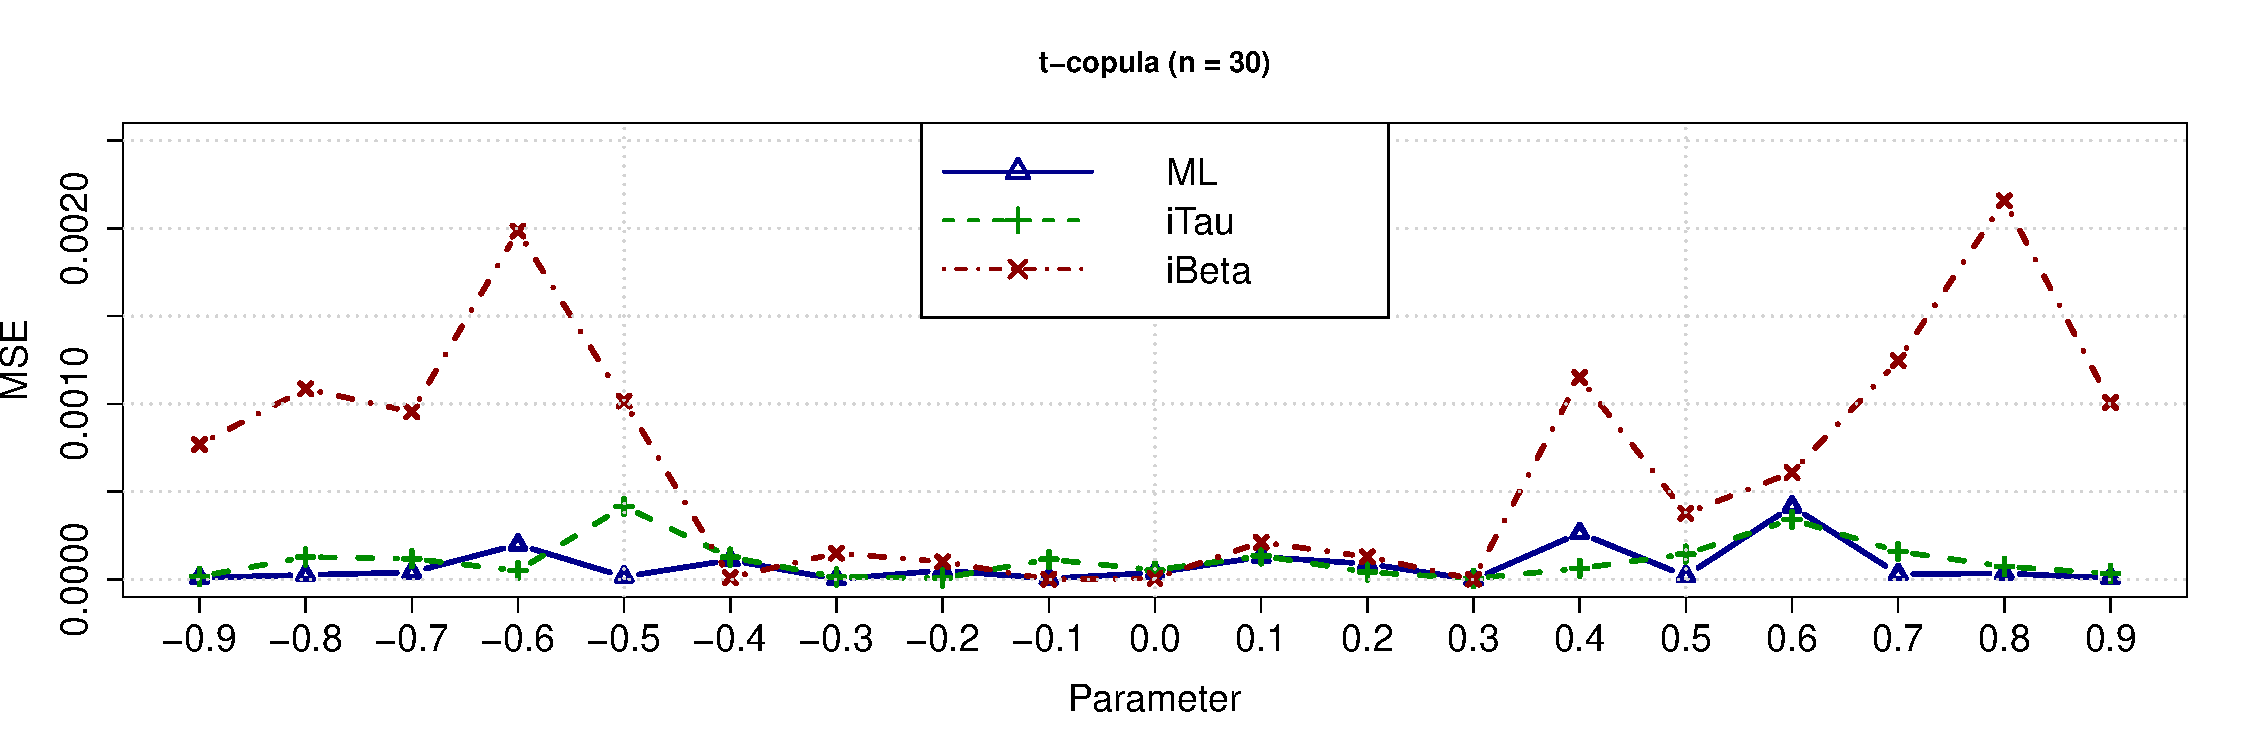
\includegraphics[trim= 0cm 1.6cm 1cm 0cm, width = .98\textwidth]{Figures/mc-plots/t30.pdf}
	}
	\hfill
	\subfloat{%
		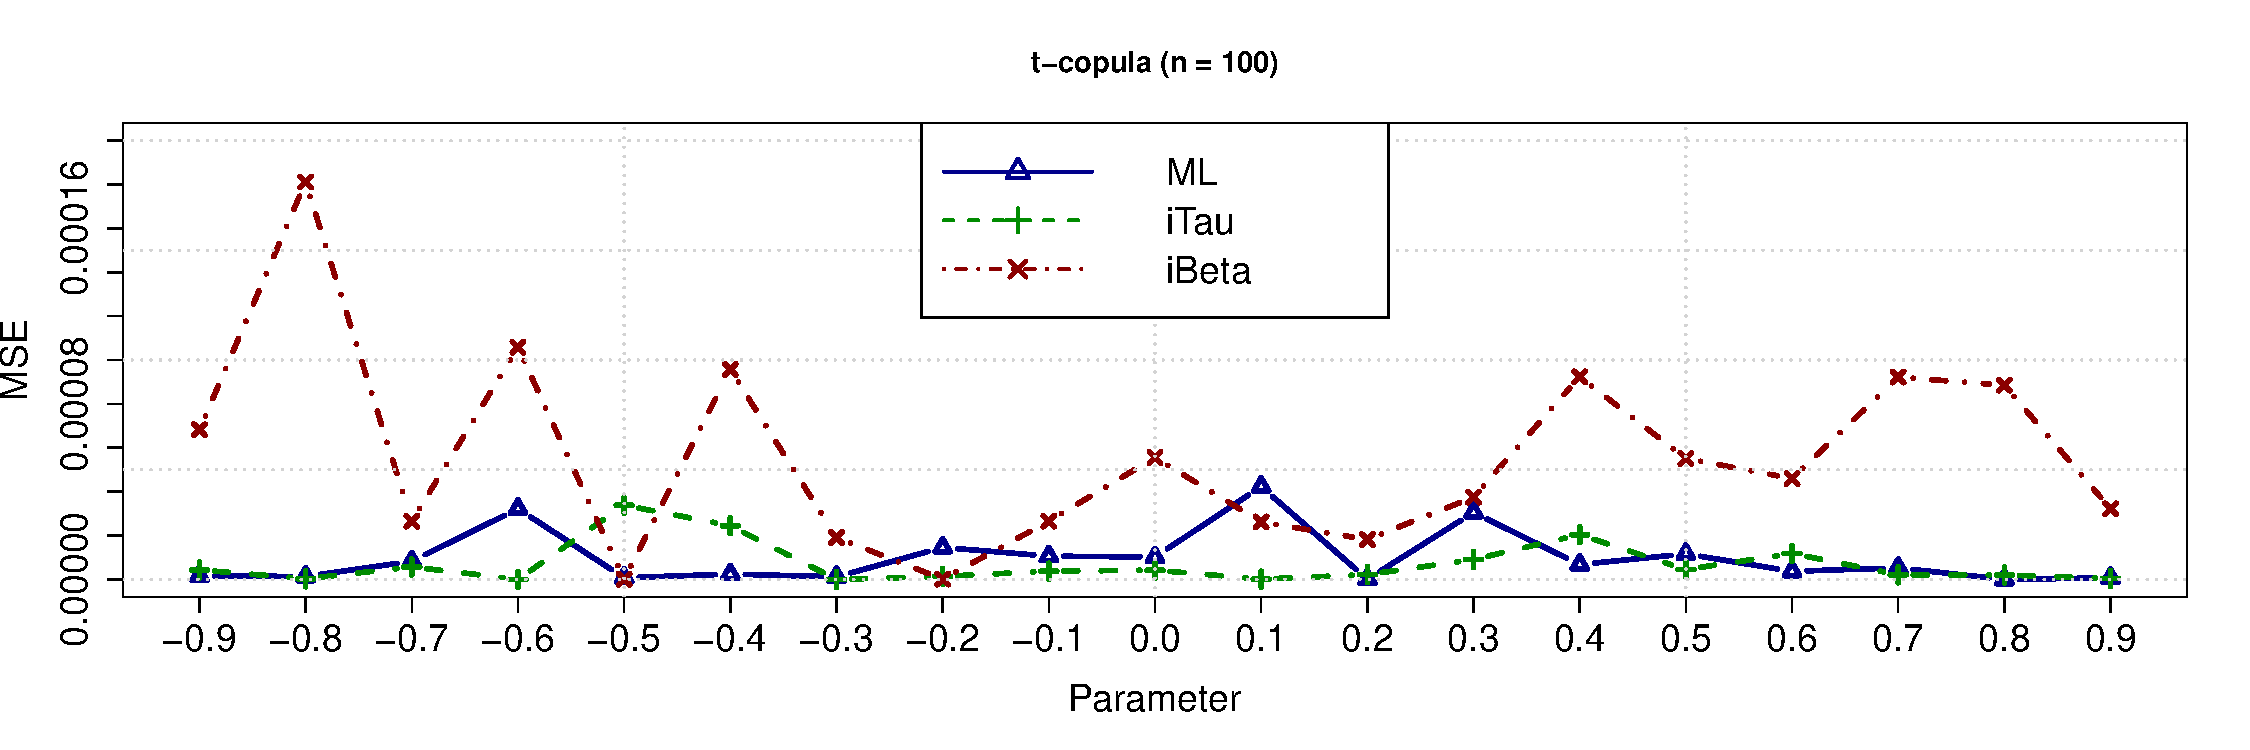
\includegraphics[trim= 0cm 1cm 1cm 0cm, width = .98\textwidth]{Figures/mc-plots/t100.pdf}
	}
	\caption[\textsc{Simulation results for Gaussian and $t$-copula}]{Mean square error for the maximum-likelihood (ML) and both inversion methods for different copulae and parameters. Sample size alternates between  $ n = \left\lbrace 30,100 \right\rbrace $ and $k = 1000$. It is assumed here that the simulated data comes from a true known copula.}
	\label{gauss_t_sim}
\end{figure}

\begin{figure}[!ht]
	\subfloat{%
		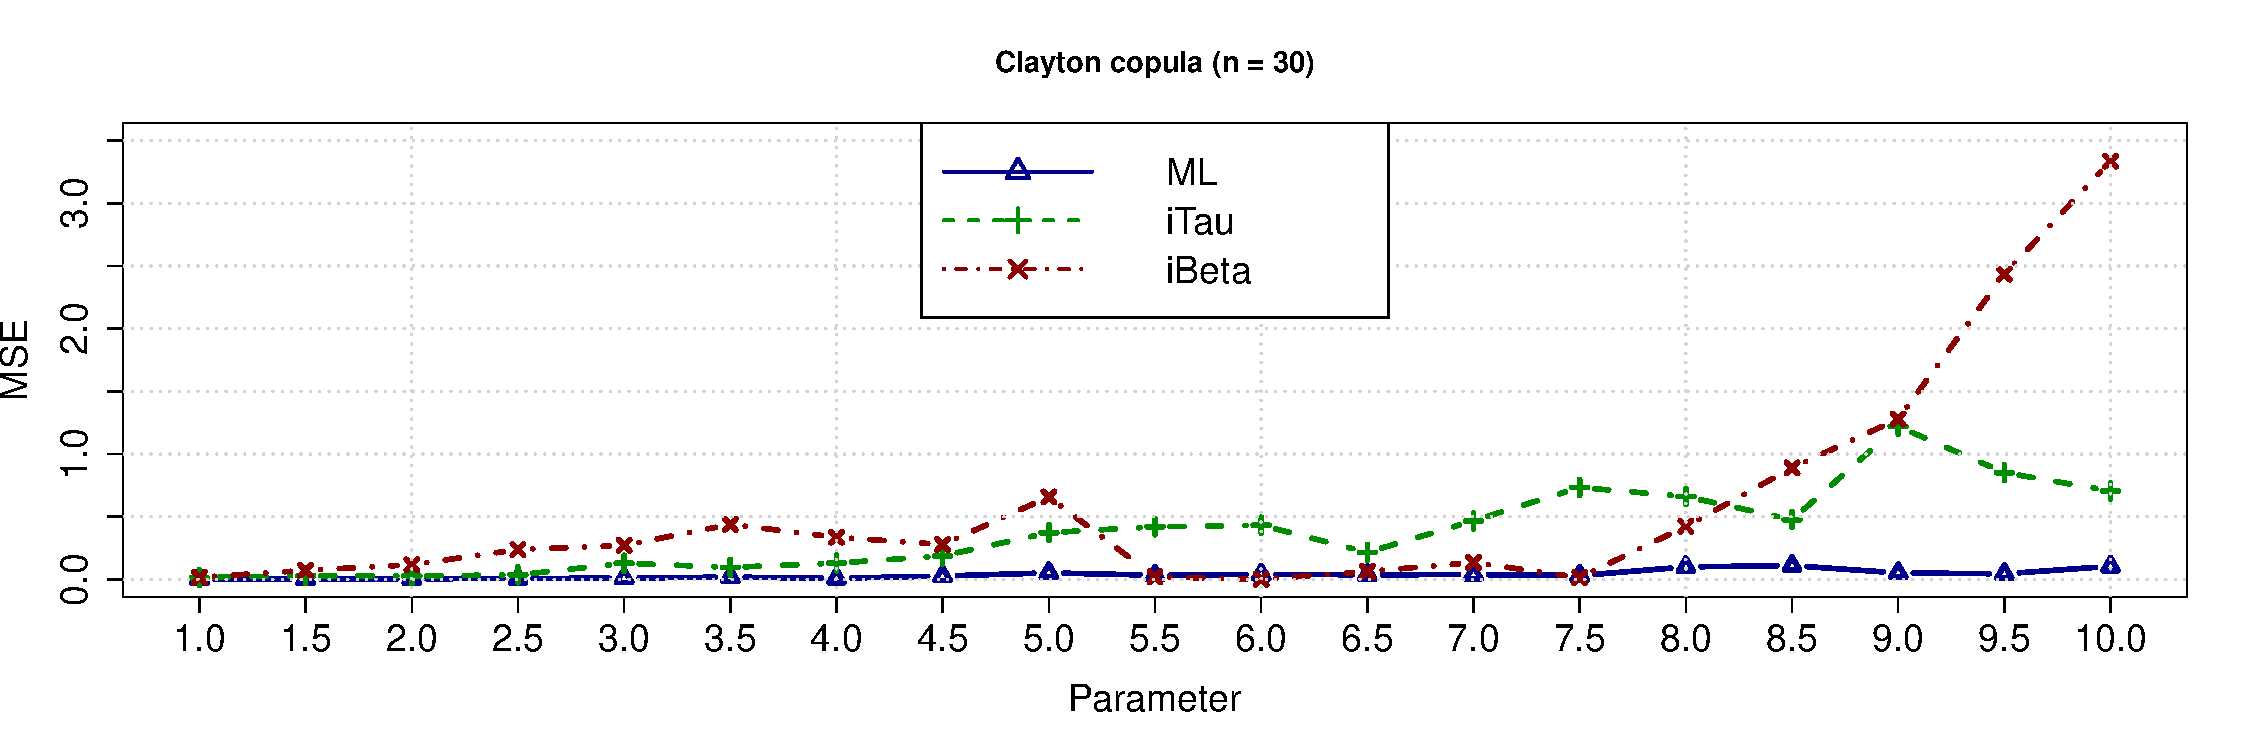
\includegraphics[trim= 0cm 1.6cm 1cm 0cm, width = .98\textwidth]{Figures/mc-plots/clayton30.pdf}
	}
	\hfill
	\subfloat{%
		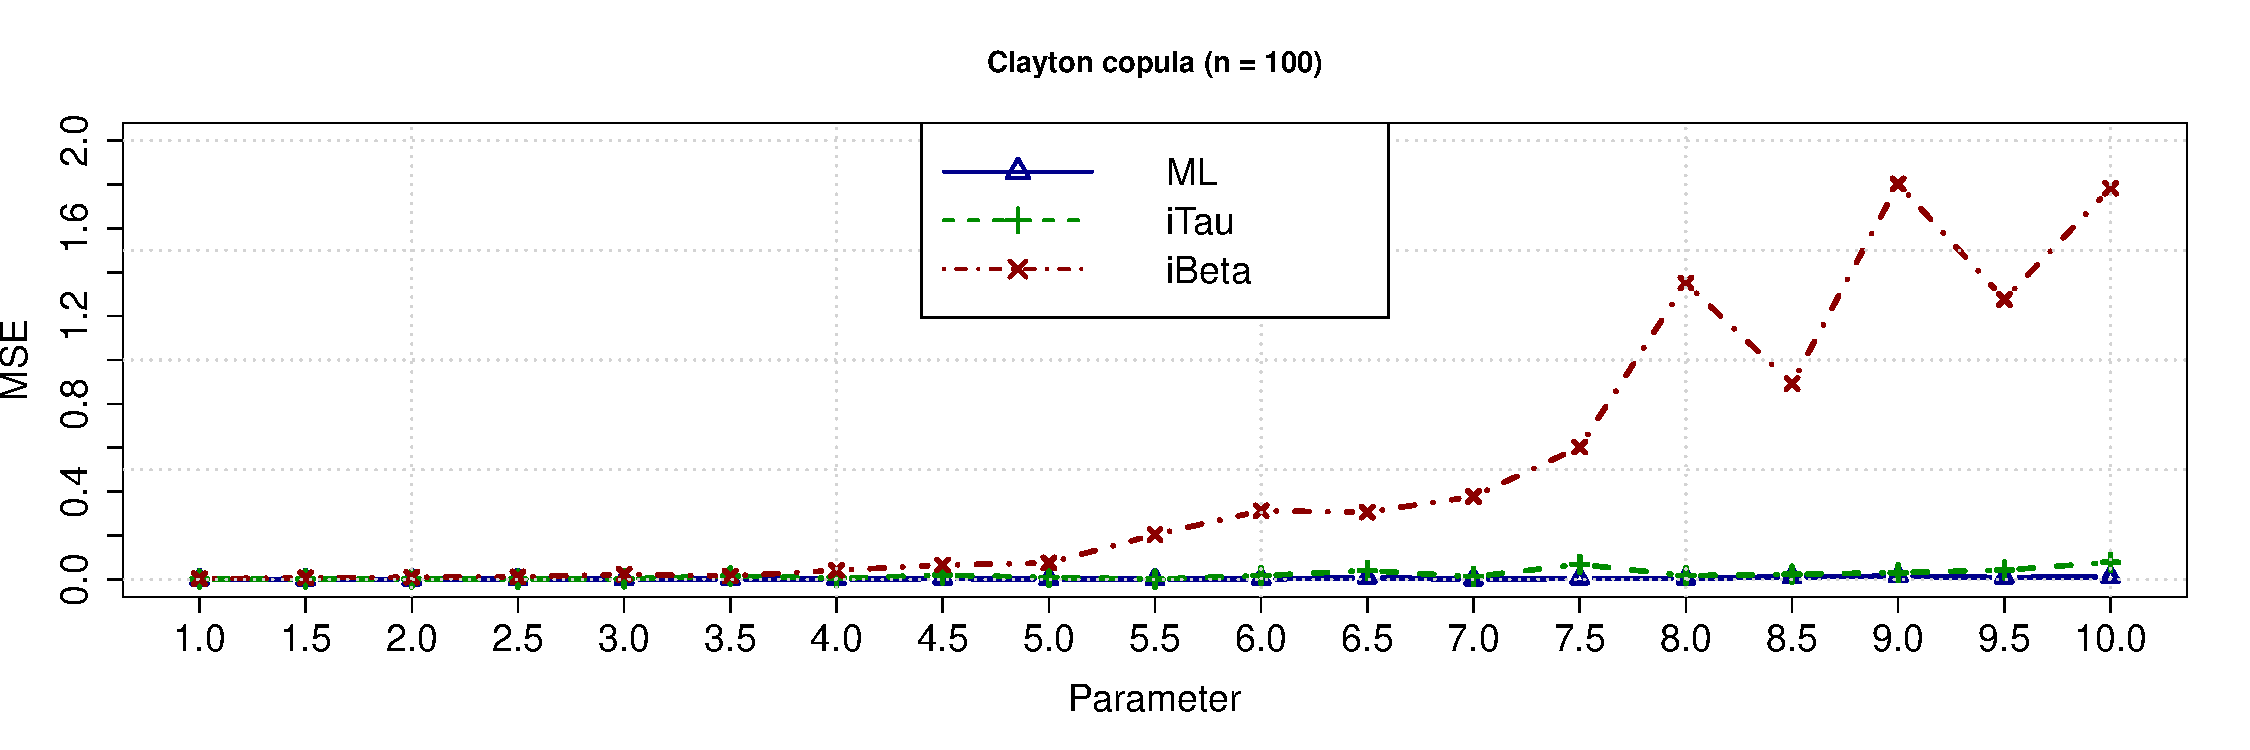
\includegraphics[trim= 0cm 1.6cm 1cm 0cm,width = .98\textwidth]{Figures/mc-plots/clayton100.pdf}
	}
	\hfill
	\subfloat{%
		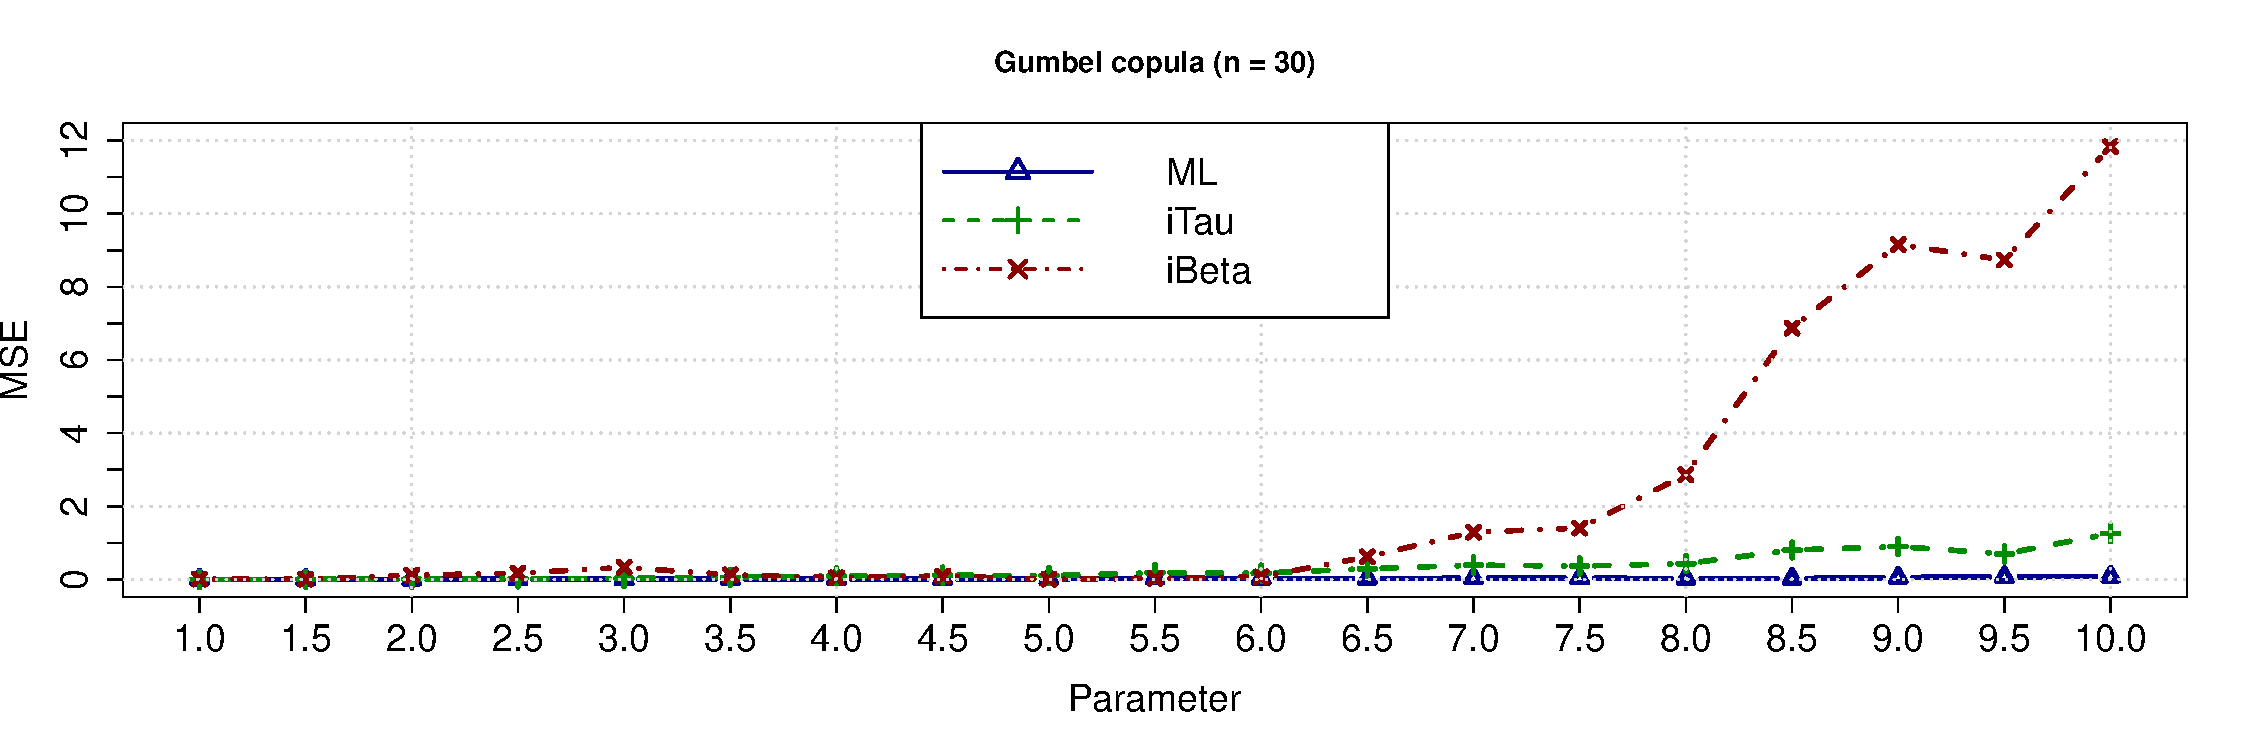
\includegraphics[trim= 0cm 1.6cm 1cm 0cm, width = .98\textwidth]{Figures/mc-plots/gumbel30.pdf}
	}
	\hfill
	\subfloat{%
		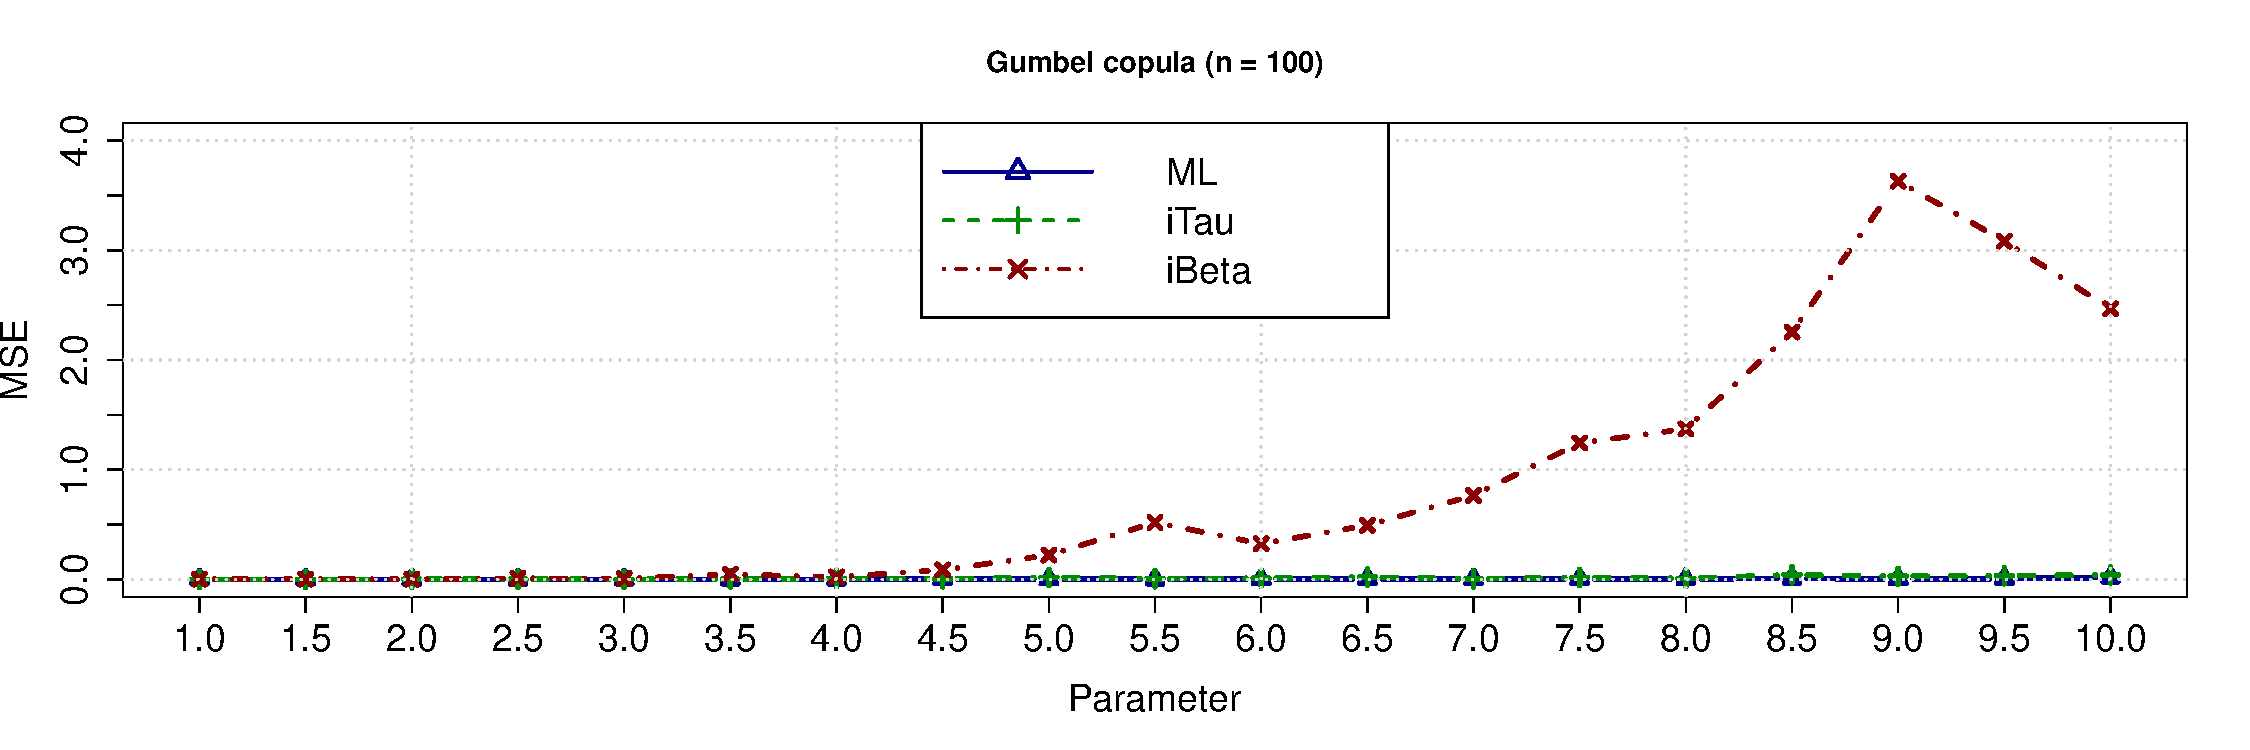
\includegraphics[trim= 0cm 1cm 1cm 0cm, width = .98\textwidth]{Figures/mc-plots/gumbel100.pdf}
	}
	\caption[\textsc{Simulation results for Clayton and Gumbel copula}]{Continuation of Figure \ref{gauss_t_sim} for the Clayton and Gumbel copula.}
	\label{clayton-gumbel-sim}
\end{figure}

\begin{figure}[!ht]
	\subfloat{%
		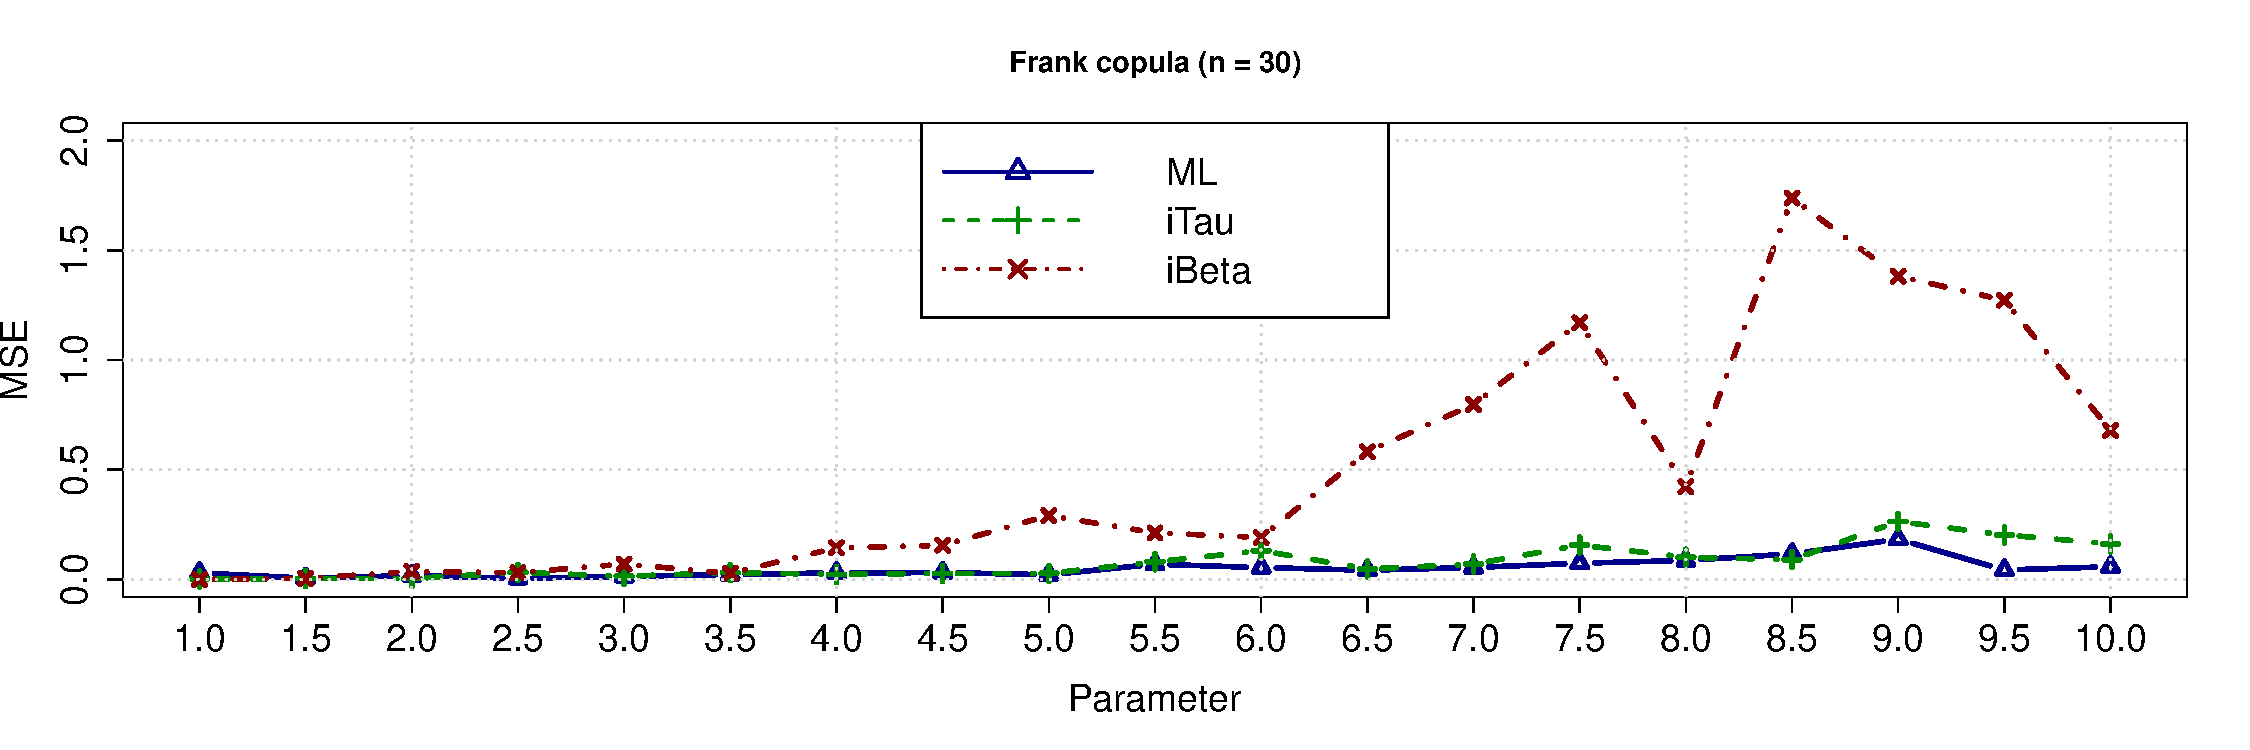
\includegraphics[trim= 0cm 1.6cm 1cm 0cm, width = .98\textwidth]{Figures/mc-plots/frank30.pdf}
	}
	\hfill
	\subfloat{%
		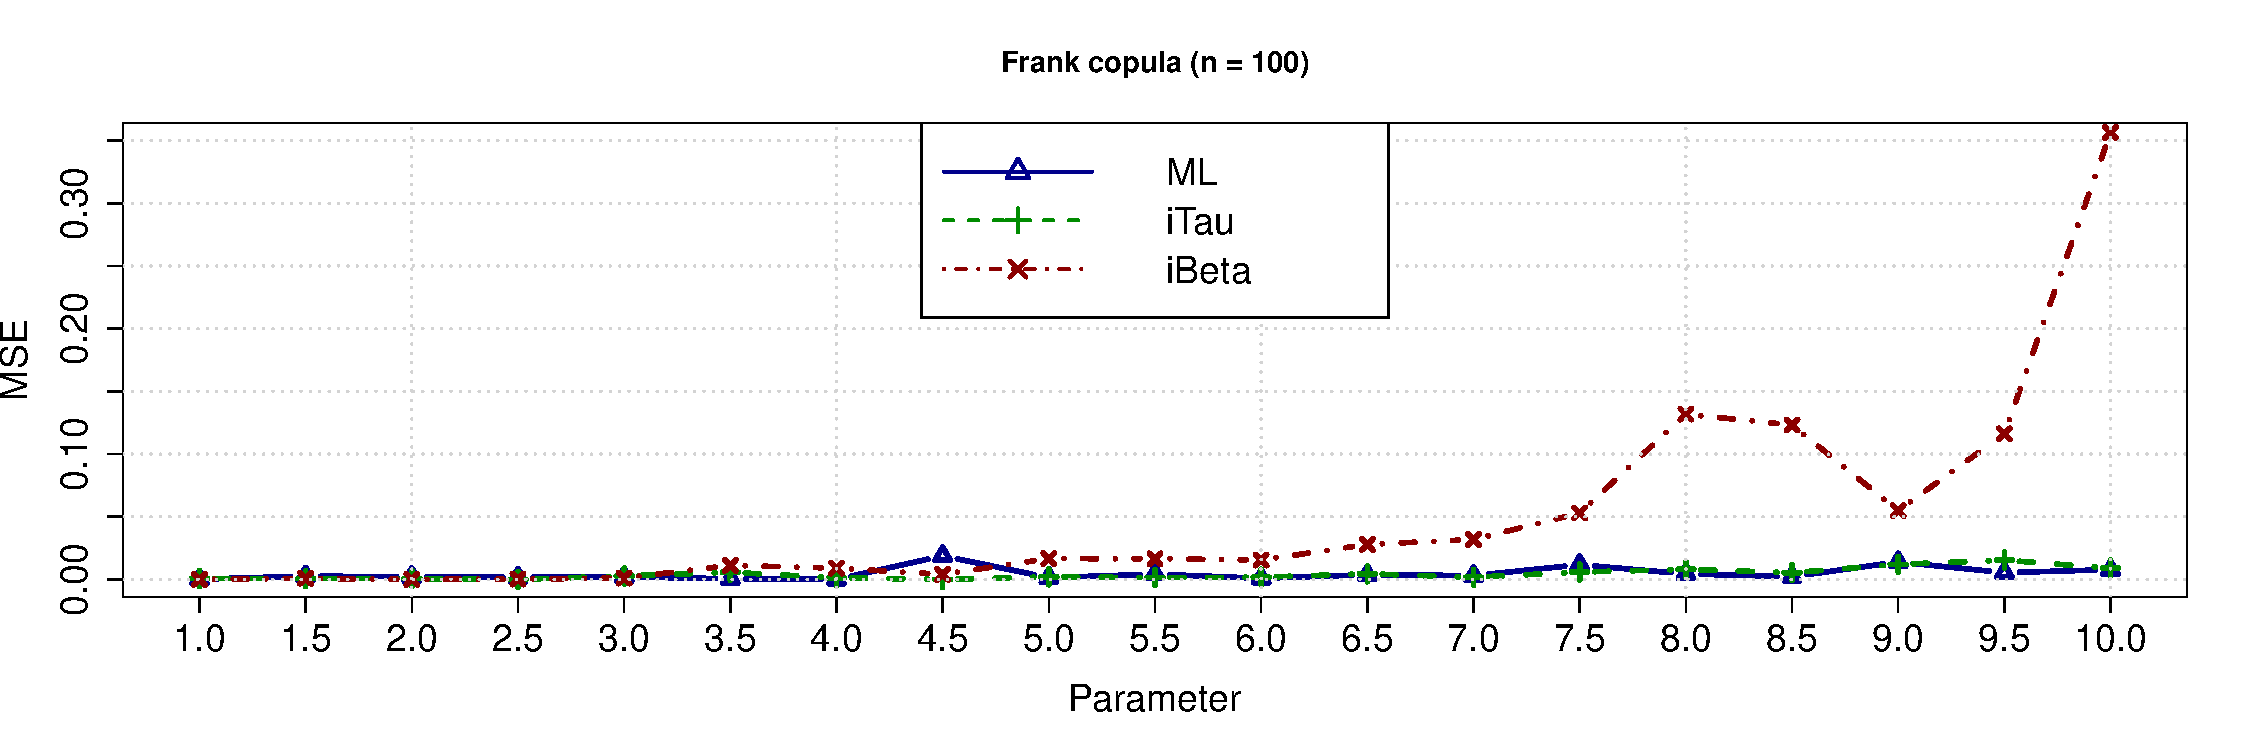
\includegraphics[trim= 0cm 1cm 1cm 0cm,width = .98\textwidth]{Figures/mc-plots/frank100.pdf}
	}
	\caption[\textsc{Simulation results for Frank copula}]{Continuation of \ref{gauss_t_sim} and \ref{clayton-gumbel-sim} for the Frank copula.}
	\label{frank-sim}
\end{figure}

\begin{table}[h!]
	\centering
{\renewcommand{\arraystretch}{1.3}
	\begin{tabular}{ll|ccc}
		Copula family             & Estimator & $\min_t$   & $\tilde{t}$ & $\max_t$   \\ \hline \hline
		\multirow{3}{*}{Gaussian} & ML        & 0.996 & 1.000      & 1.051 \\
		& iTau      & 0.146 & 0.147  & 0.148 \\
		& iBeta     & 0.182 & 0.183  & 0.185 \\ \hline
		\multirow{3}{*}{t}        & ML        & 0.989 & 1.000      & 1.045 \\
		& iTau      & 0.032 & 0.032  & 0.033 \\
		& iBeta     & 0.035 & 0.035  & 0.036 \\ \hline
		\multirow{3}{*}{Clayton}  & ML        & 0.992 & 1.000      & 1.006 \\
		& iTau      & 0.152 & 0.155  & 0.157 \\
		& iBeta     & 0.247 & 0.248  & 0.251 \\ \hline
		\multirow{3}{*}{Gumbel}   & ML        & 0.999 & 1.000      & 1.002 \\
		& iTau      & 0.113 & 0.114  & 0.114 \\
		& iBeta     & 0.139 & 0.140  & 0.141 \\ \hline
		\multirow{3}{*}{Frank}    & ML        & 0.997 & 1.000      & 1.006 \\
		& iTau      & 0.922 & 0.923  & 0.925 \\
		& iBeta     & 0.909 & 0.910  & 0.917
	\end{tabular}
}
\caption[Relative computation time per estimator and copula for parameter estimation.]{Relative computation time per copula and estimator. For the benchmark I calculated the average time it takes the algorithm to converge to a parameter. I use $n = 100$ and $k = 5000$.}
\label{rel-comp-time-est}
\end{table}

\subsection{Estimator choice for copula selection}

Figures \ref{copSelect-gauss-t} and \ref{copSelect-gumbel-frank} depict the accuracy of each estimator copula and parameter for the selection process based the AIC for $ n = \left\lbrace 30,100 \right\rbrace $ and $k = 100$. Surprisingly, all estimators seem to perform equally in terms of selecting a copula, given a set of data. The difference in computation time between the estimators from Table \ref{comp-time-seletion}, however, is noteworthy. Even for the smallest sample size $n = 30$, there is no notable difference in accuracy across all copulae and parameters, yet the inversion methods are at least 16 times faster than maximum-likelihood. This is most likely due to skipped optimization process for the inversion methods, as no first- or second-order derivatives need to be calculated.



\begin{figure}[t]
	\subfloat{%
		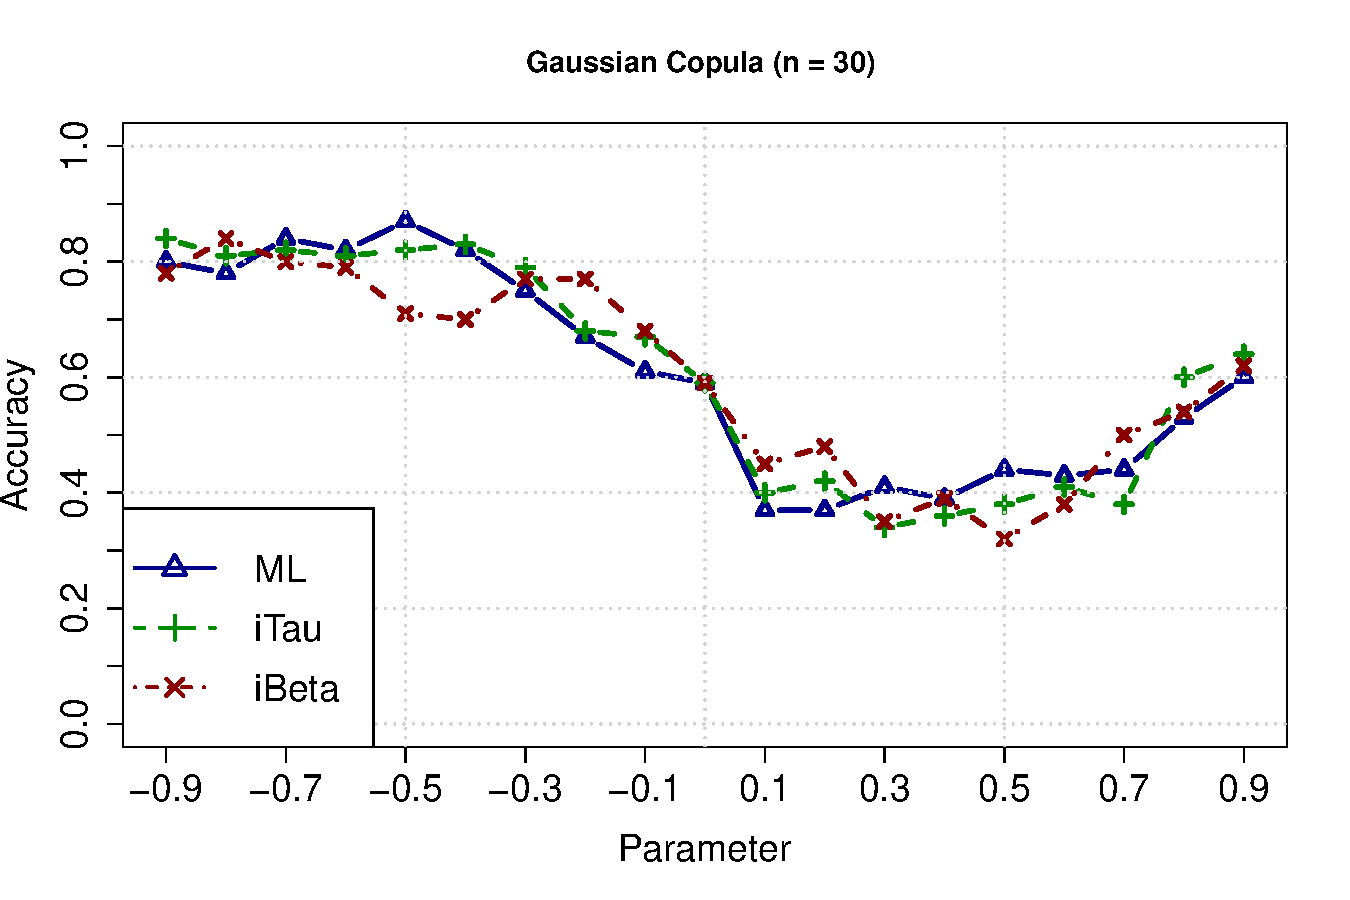
\includegraphics[trim= 0cm 0cm 1cm .7cm,clip=true, width = .48\textwidth]{Figures/mc-copSelection/gaussian-select30.pdf}
	}
	\hfill
	\subfloat{%
		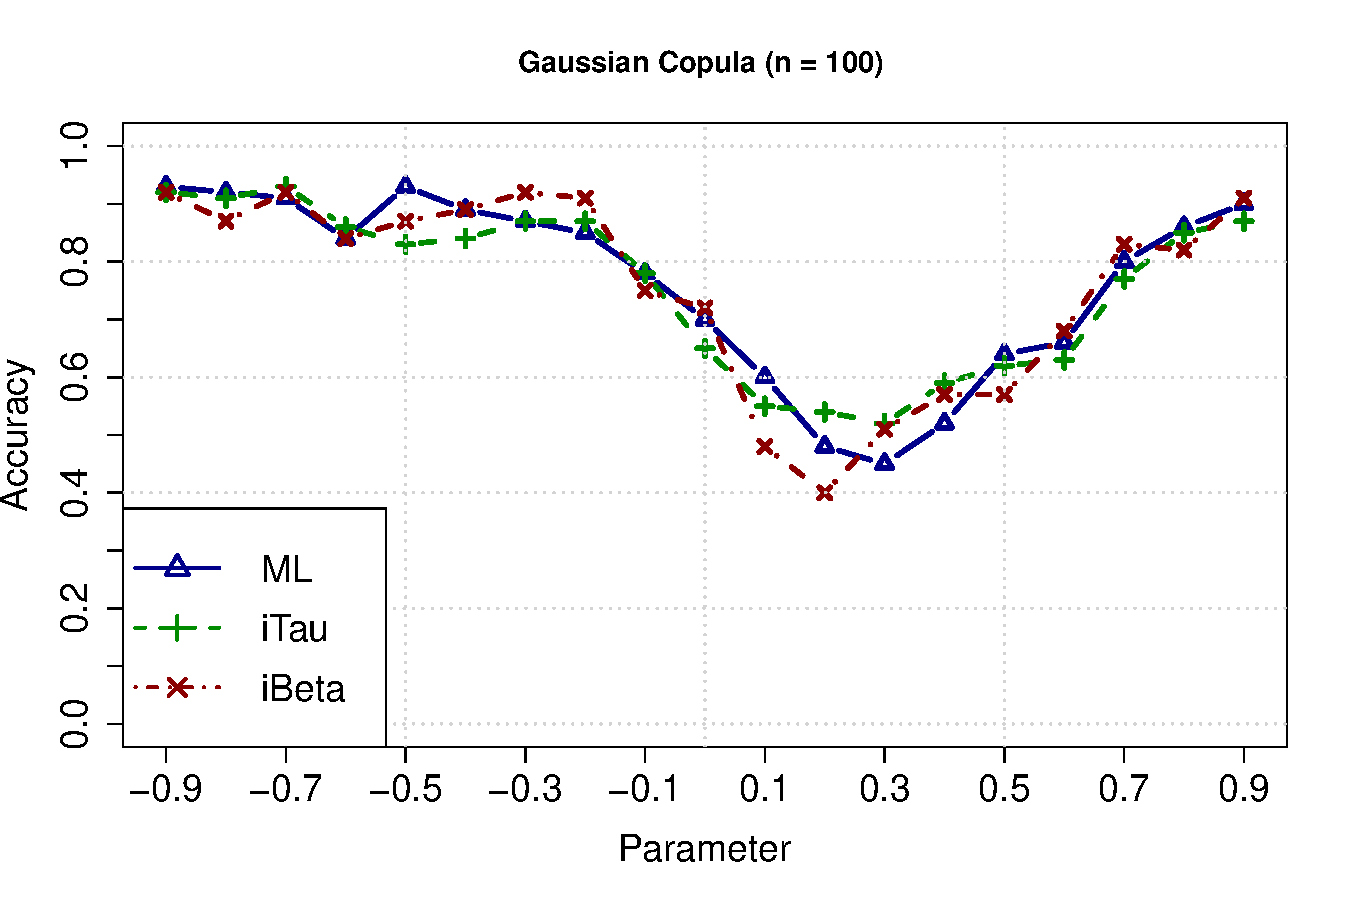
\includegraphics[trim= 0cm 0cm 1cm .7cm,clip=true,width = .48\textwidth]{Figures/mc-copSelection/gaussian-select100.pdf}
	}
	\hfill
	\subfloat{%
		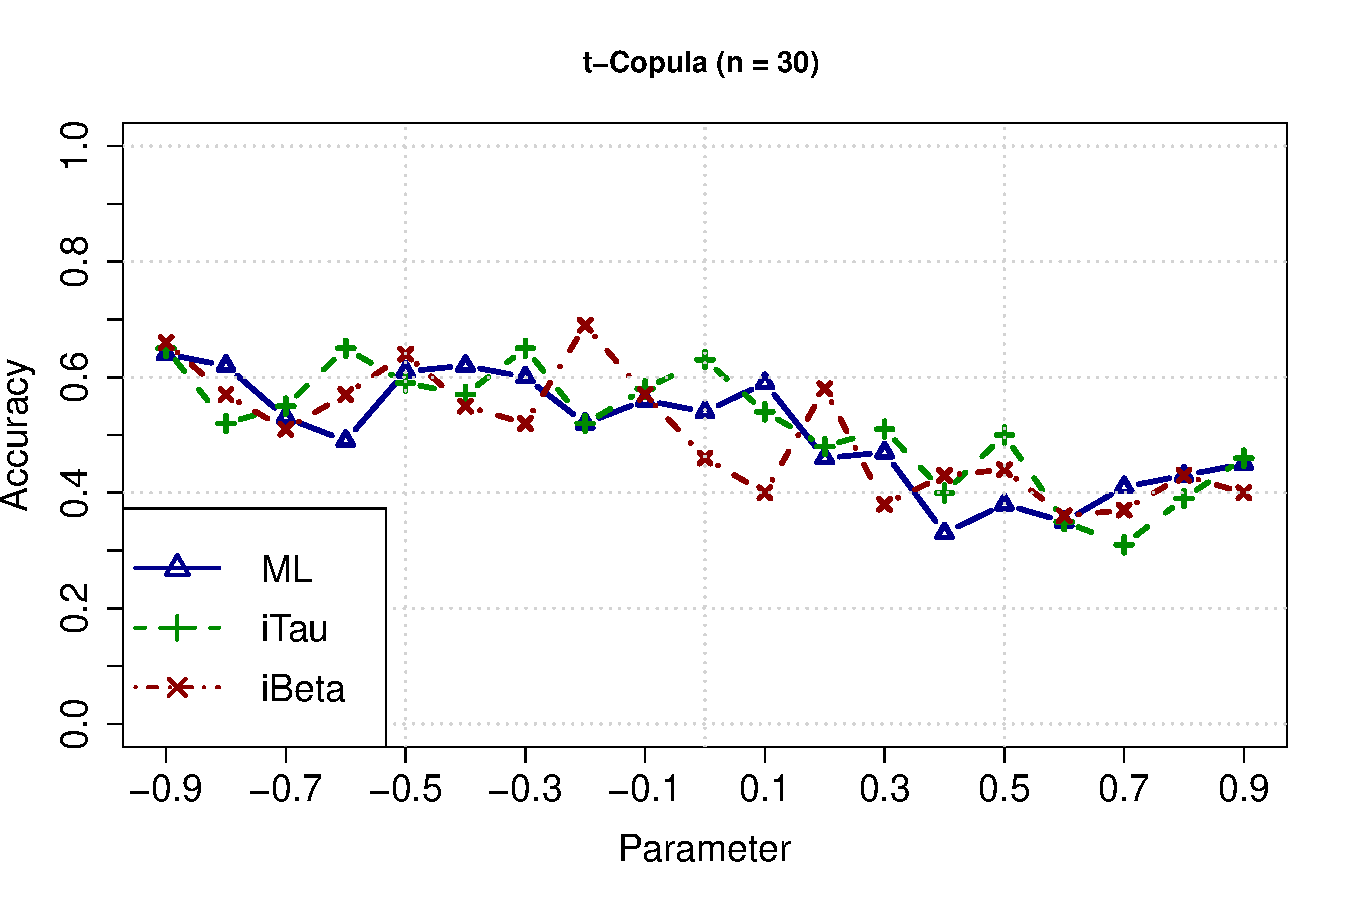
\includegraphics[trim= 0cm 0cm 1cm .7cm,clip=true,width = .48\textwidth]{Figures/mc-copSelection/t-select30.pdf}
	}
	\hfill
	\subfloat{%
		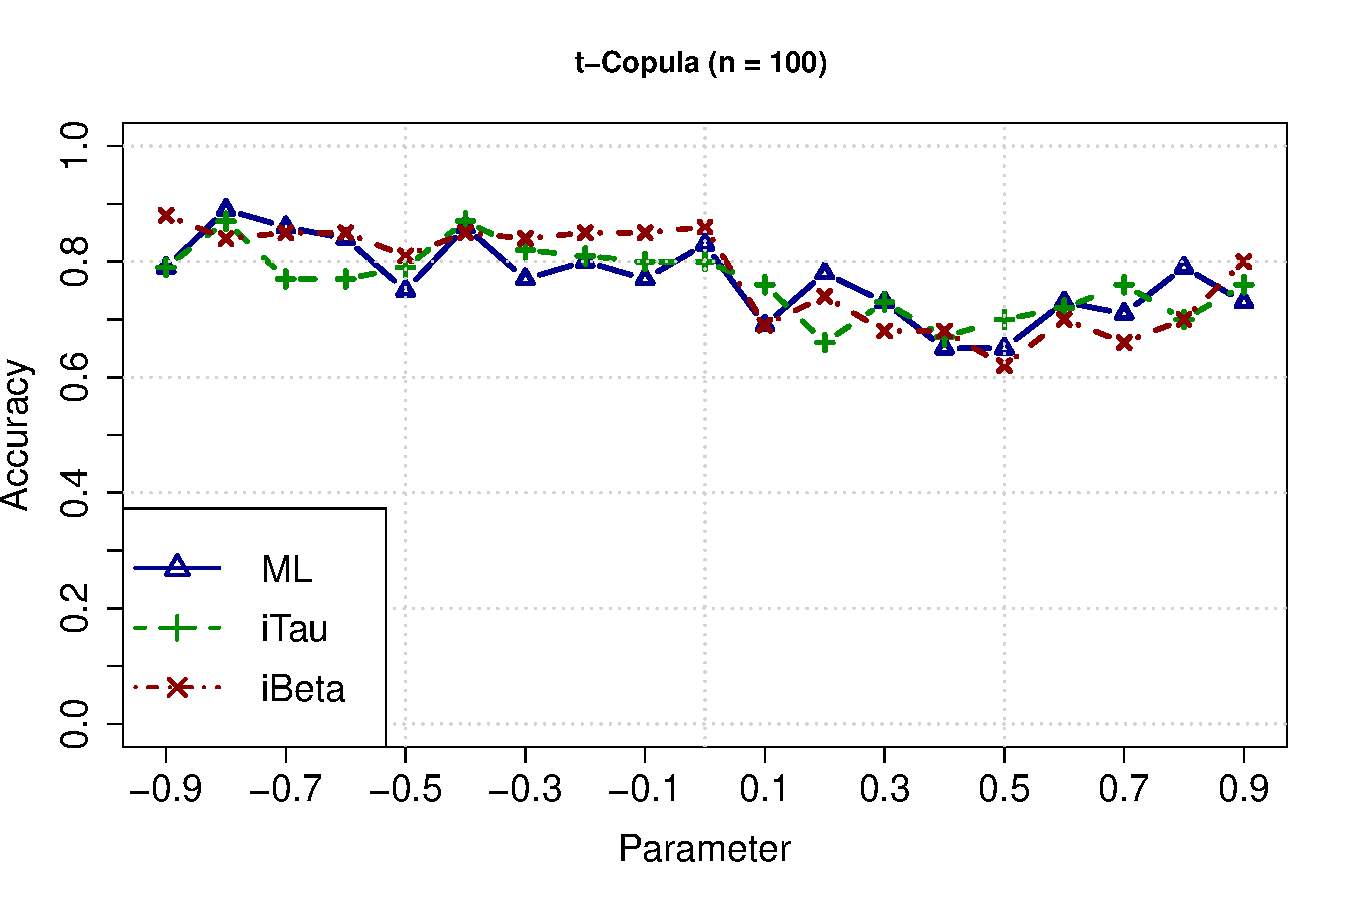
\includegraphics[trim= 0cm 0cm 1cm .7cm,clip=true,width = .48\textwidth]{Figures/mc-copSelection/t-select100.pdf}
	}
	\hfill
	\subfloat{%
		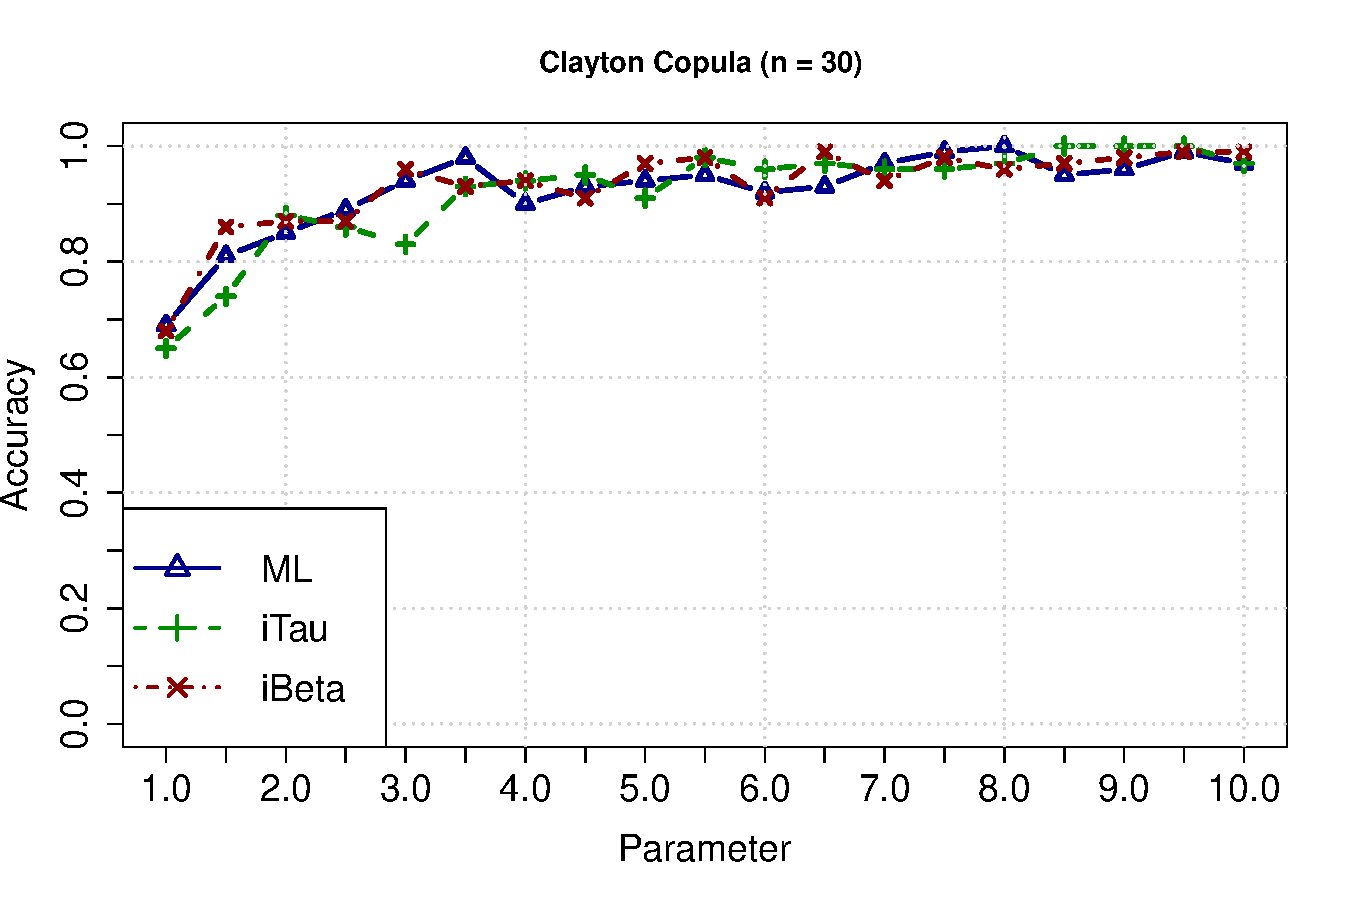
\includegraphics[trim= 0cm 0cm 1cm .7cm,clip=true,width = .48\textwidth]{Figures/mc-copSelection/clayton-select30.pdf}
	}
	\hfill
	\subfloat{%
		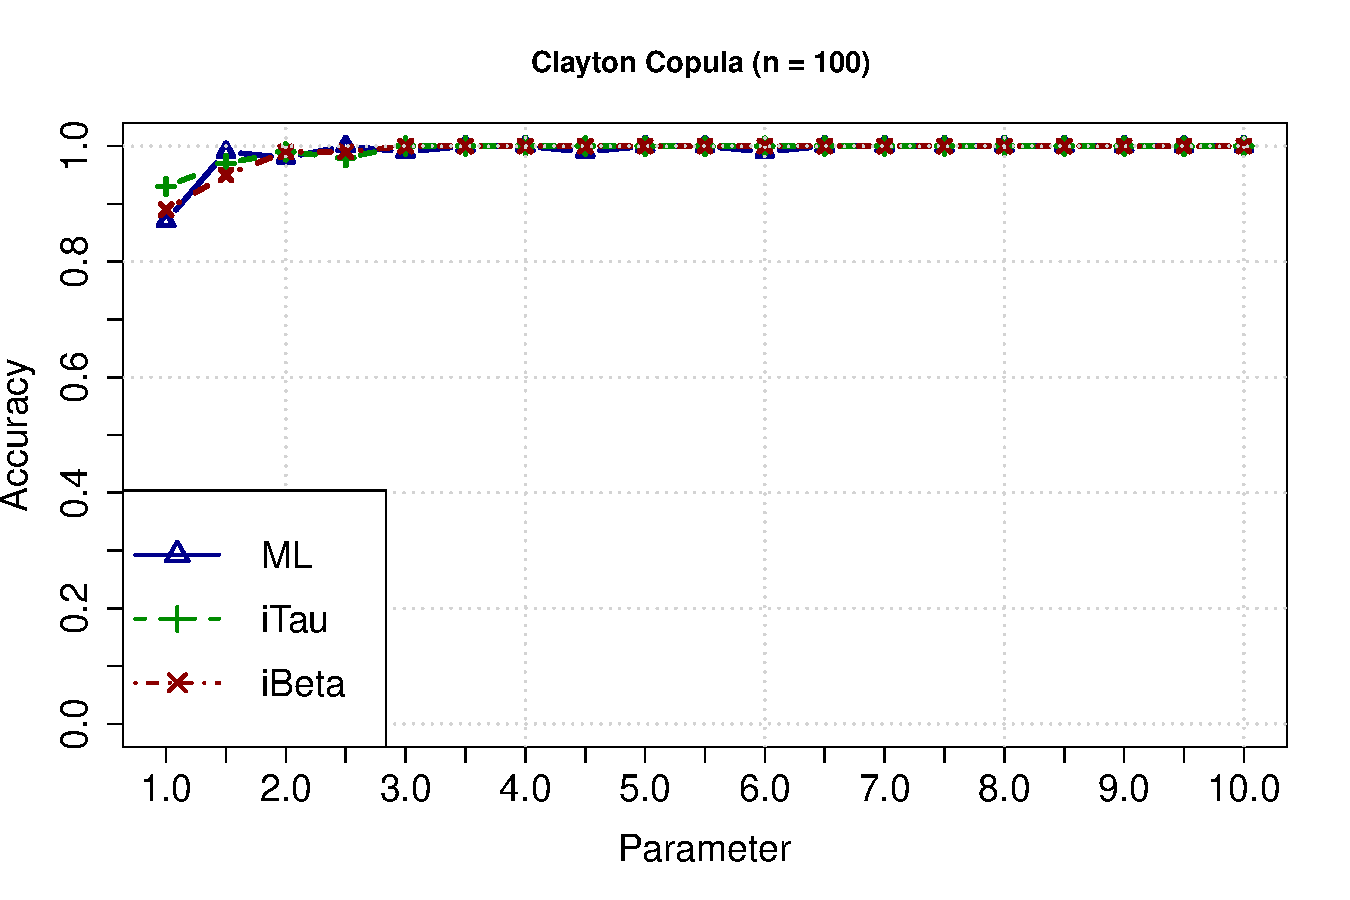
\includegraphics[trim= 0cm 0cm 1cm .7cm,clip=true,width = .48\textwidth]{Figures/mc-copSelection/clayton-select100.pdf}
	}
	\caption[\textsc{Accuracy of copula selection for different estimators / Gaussian, $t$ and Clayton copula}]{Accuracy of copula selection for different estimators with $ n = \left\lbrace 30,100 \right\rbrace $ and $k = 100$. Shown is the percentage of correct specifications per estimator, copula and parameter. This Figure images the behavior for the Gaussian, $t$, and Clayton copula.}
	\label{copSelect-gauss-t}
\end{figure}

\begin{figure}[t]
	\subfloat{%
		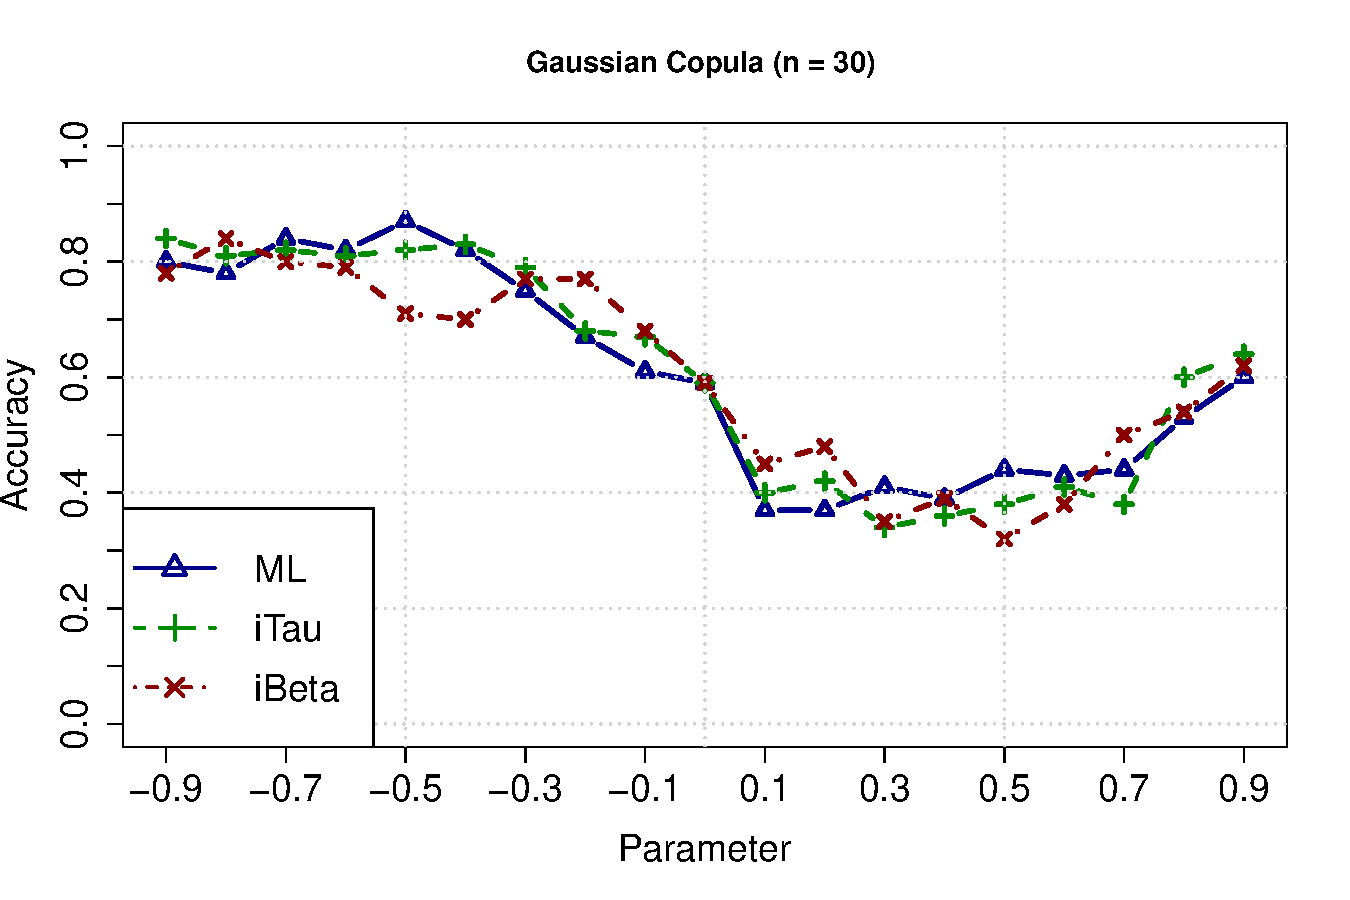
\includegraphics[trim= 0cm 0cm 1cm .7cm,clip=true, width = .48\textwidth]{Figures/mc-copSelection/gaussian-select30.pdf}
	}
	\hfill
	\subfloat{%
		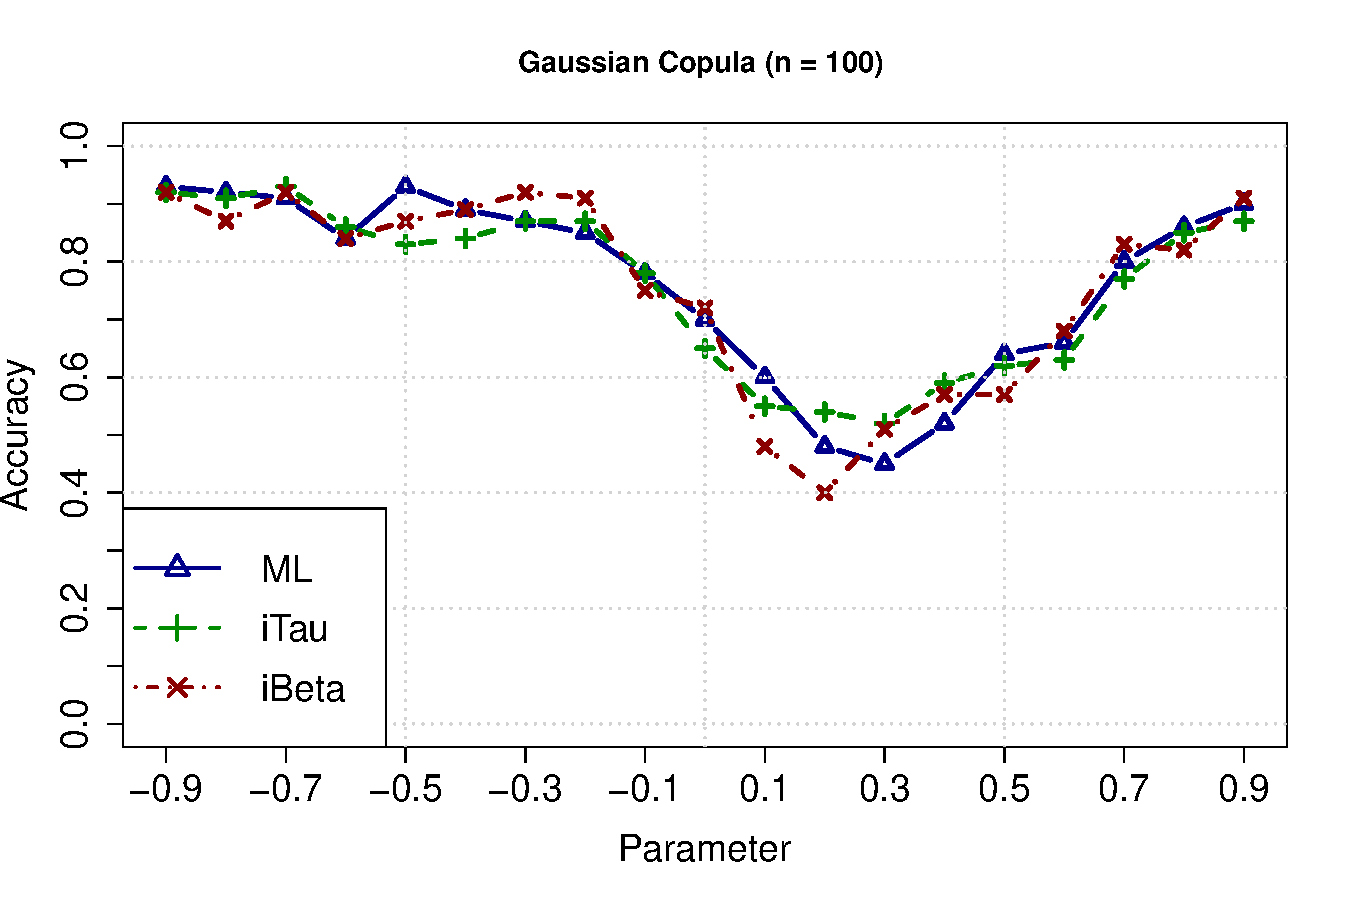
\includegraphics[trim= 0cm 0cm 1cm .7cmm,clip=true,width = .48\textwidth]{Figures/mc-copSelection/gaussian-select100.pdf}
	}
	\hfill
	\subfloat{%
		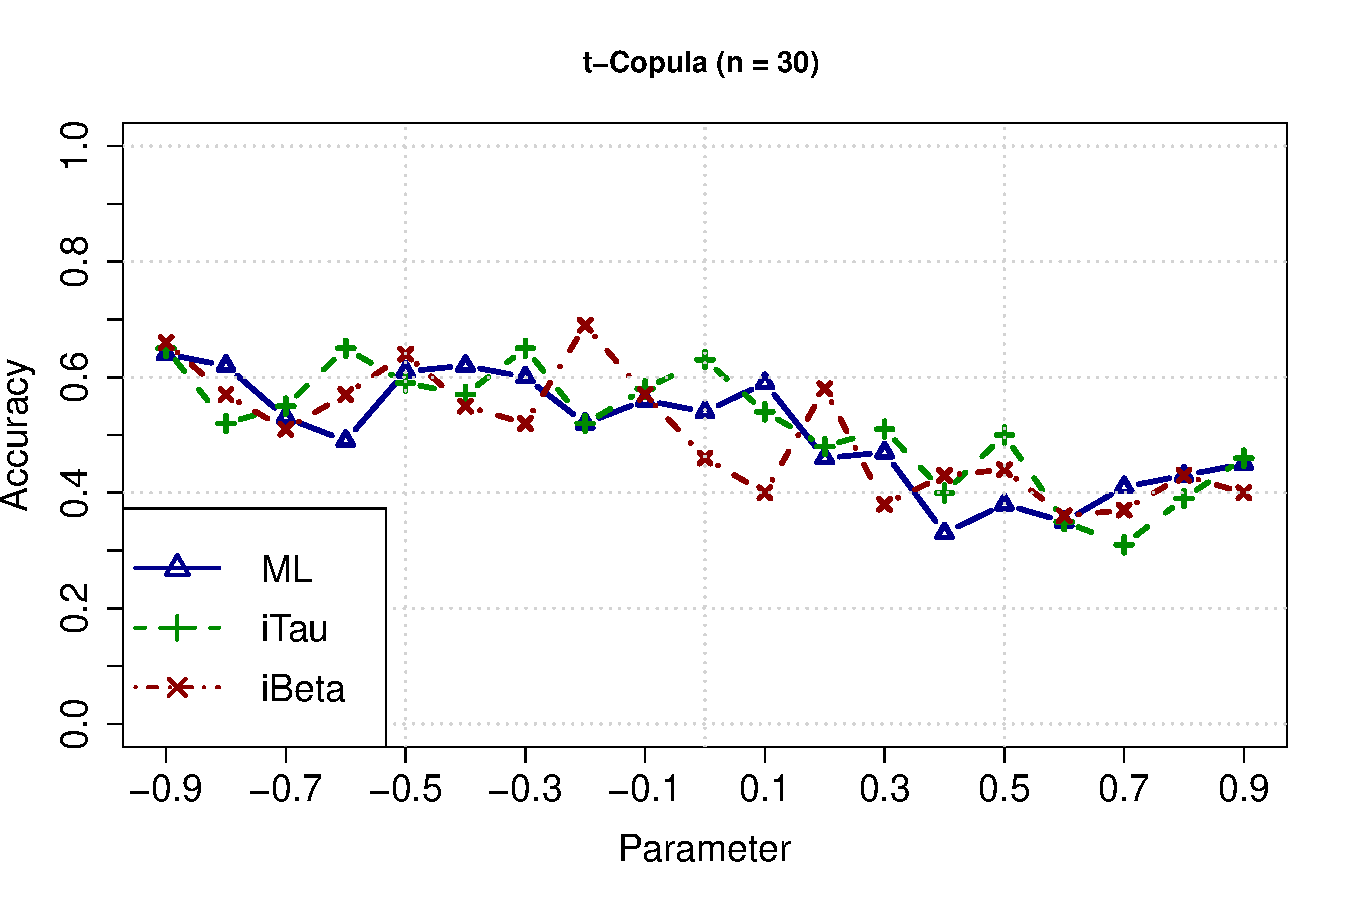
\includegraphics[trim= 0cm 0cm 1cm .7cm,clip=true,width = .48\textwidth]{Figures/mc-copSelection/t-select30.pdf}
	}
	\hfill
	\subfloat{%
		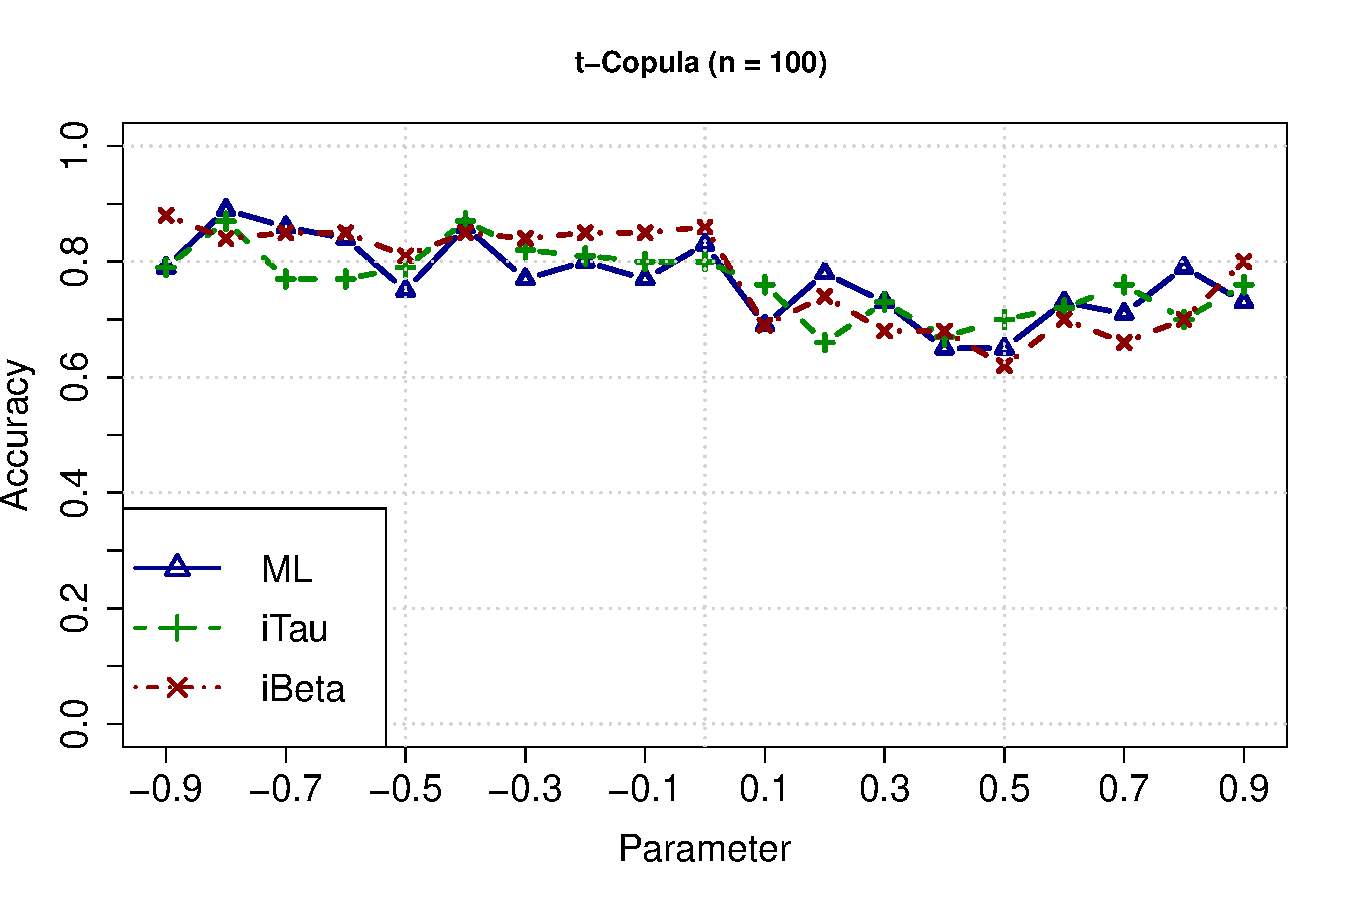
\includegraphics[trim= 0cm 0cm 1cm .7cm,clip=true,width = .48\textwidth]{Figures/mc-copSelection/t-select100.pdf}
	}
	\caption[\textsc{Accuracy of copula selection for different estimators / Gumbel and Frank copula}]{Continuation of Figure \ref{copSelect-gauss-t} for the Gumbel and Frank copula.}
	\label{copSelect-gumbel-frank}
\end{figure}


\begin{table}[h!]
	\centering
{\renewcommand{\arraystretch}{1.3}
	\begin{tabular}{ll|ccc}
		Copula family             & Estimator & $\min_t$   & $\tilde{t}$ & $\max_t$   \\ \hline \hline
		\multirow{3}{*}{Gaussian} & ML        & 0.666 & 1      & 3.706 \\
		& iTau      & 0.051 & 0.053  & 0.115 \\
		& iBeta     & 0.050 & 0.051  & 0.112 \\ \hline
		\multirow{3}{*}{t}        & ML        & 0.647 & 1      & 3.576 \\
		& iTau      & 0.050 & 0.051  & 0.159 \\
		& iBeta     & 0.048 & 0.049  & .0125 \\ \hline
		\multirow{3}{*}{Clayton}  & ML        & 0.606 & 1      & 2.936 \\
		& iTau      & 0.040 & 0.041  & 0.090 \\
		& iBeta     & 0.039 & 0.040  & 0.084 \\ \hline
		\multirow{3}{*}{Gumbel}   & ML        & 0.643 & 1      & 2.638 \\
		& iTau      & 0.059 & 0.061  & 0.086 \\
		& iBeta     & 0.058 & 0.059  & 0.104 \\ \hline
		\multirow{3}{*}{Frank}    & ML        & 0.670 & 1      & 3.288 \\
		& iTau      & 0.044 & 0.045  & 0.100 \\
		& iBeta     & 0.042 & 0.043  & 0.076
	\end{tabular}
}
\caption[Relative computation time per copula and estimator for copula selection]{Relative computation time per copula and estimator for the selection process. Time is measured relative to the median time it takes the maximum likelihood estimator in combination with the AIC to find an optimal copula. $n$ has been set to $100$ and $k = 1000$. }
\label{comp-time-seletion}
\end{table}

\section{Conclusion}

This study compared the performance and accuracy of three different estimators regarding parameter estimation and selection of copulae. Concerning the first one, the results of previous studies could be reproduced, finding that for accurate estimation of a copula's parameter the maximum likelihood estimator remains the mean of choice. Both moment based estimators, especially Blomqvist's Beta are significantly worse in estimating, however, are considerably faster computationally. Hence, one could use those estimators to perform a quick-and-dirty estimation to find a starting value for a subsequent ML estimation. This poses the interesting question of how much more efficient such a procedure would be in comparison to only use ML.

In a second step a fast procedure for selecting copulae could be found. The accuracy when selecting copulae remains almost equal across all copulae, parameters and sample sizes for every estimator. In terms of algorithmic complexity, the moment-based estimators stand out, as they only need a fraction of the time ML needs to select a copula from arbitrarily generated data. Therefore, it seems reasonable to prefer those over ML, especially in large sample size or big-data environments. The \verb*|R| workspace and functions can be provided upon request.

With over $855,000$ parameter estimations and around $57,000$ copula selections computed in this study, it counts to the more comprehensive ones carried out so far, yet there are also drawbacks. I only implemented the selection process for five copulae and three estimators, so it would be an interesting task to realize the selection algorithm for the remaining copulae and also test its performance. A real-world application putting the algorithm to use is also pending. 

%----------------------------------------------------------------------------------------
%	THESIS CONTENT - APPENDICES
%----------------------------------------------------------------------------------------

\appendix %The following "chapters" are Appendices


% Appendix A

\chapter{Appendix} % Main appendix title

\label{AppendixA} % For referencing this appendix elsewhere, use \ref{AppendixA}


\section{Proof of \ref{tau-copula}}

In \ref{emp-kendall} we discussed an empirical version of Kendall's Tau. For this proof we use the population analogue, given by

\begin{equation*}
	\tau\left(X_{1}, X_{2}\right)=P\left[ \left(X_{11}-X_{21}\right)\left(X_{12}-X_{22}\right)>0\right] -P\left[ \left(X_{11}-X_{21}\right)\left(X_{12}-X_{22}\right)<0\right] ,
\end{equation*}
%
where $(X_{11},X_{12})$ and $(X_{21},X_{22})$ are independent copies of $(X_1,X_2)$.
%
Now, based on 

\begin{equation*}
	P\left[ \left(X_{11}-X_{21}\right)\left(X_{12}-X_{22}\right)>0\right] =1-P\left[ \left(X_{11}-X_{21}\right)\left(X_{12}-X_{22}\right)<0\right],
\end{equation*}
%
one can write $\tau=2 P\left(\left(X_{11}-X_{21}\right)\left(X_{12}-X_{22}\right)>0\right)-1$.
%
Furthermore, using 

\begin{equation*}
	{\scriptstyle P\left[ \left(X_{11}-X_{21}\right)\left(X_{12}-X_{22}\right)>0\right] =P\left(X_{11}>X_{21}, X_{12}>X_{22}\right)+P\left(X_{11}<X_{21}, X_{12}<X_{22}\right)}
\end{equation*}
%
and the transformation $u_{1}:=F_{1}\left(x_{1}\right)$ and $u_{2}:=F_{2}\left(x_{2}\right)$ one obtains:

\begin{equation*}
	\begin{aligned}
		P\left(X_{11}>X_{21}, X_{12}>X_{22}\right) &=P\left(X_{21}<X_{11}, X_{22}<X_{12}\right) \\
		&=\int_{-\infty}^{\infty} \int_{-\infty}^{\infty} P\left(X_{21}<x_{1}, X_{22}<x_{2}\right) d C\left(F_{1}\left(x_{1}\right), F_{2}\left(x_{2}\right)\right) \\
		&=\int_{-\infty}^{\infty} \int_{-\infty}^{\infty} C\left(F_{1}\left(x_{1}\right), F_{2}\left(x_{2}\right)\right) d C\left(F_{1}\left(x_{1}\right), F_{2}\left(x_{2}\right)\right) \\
		&=\int_{0}^{1} \int_{0}^{1} C\left(u_{1}, u_{2}\right) d C\left(u_{1}, u_{2}\right).
	\end{aligned}
\end{equation*}
%
The same can be shown for 

\begin{equation*}
		P\left(X_{11}<X_{21}, X_{12}<X_{22}\right)=\int_{0}^{1} \int_{0}^{1}\left[1-u_{1}-v_{1}+C\left(u_{1}, u_{2}\right)\right] d C\left(u_{1}, u_{2}\right),
\end{equation*}
%
and as $C$ is the distribution function of $U_j := F_j(X_j)$ for $j = 1,2$ with mean $1/2$ one obtains

\begin{equation*}
	\begin{aligned}
		P\left(X_{11}<X_{21}, X_{12}<X_{22}\right) &=1-\frac{1}{2}-\frac{1}{2}+\int_{0}^{1} \int_{0}^{1} C\left(u_{1}, u_{2}\right) d C\left(u_{1}, u_{2}\right) \\
		&=\int_{0}^{1} \int_{0}^{1} C\left(u_{1}, u_{2}\right) d C\left(u_{1}, u_{2}\right)
	\end{aligned}.
\end{equation*}
%
Therefore, 

\begin{equation}
	\tau=-1+4 \int_{[0,1]^{2}} C\left(u_{1}, u_{2}\right) \mathrm{d} C\left(u_{1}, u_{2}\right).
\end{equation}

\section{Proof of \ref{beta-copula}}

This proof is taken from \citet{genest2013copula}, but also repeated here for completeness. For two random variables $X$ and $Y$ with their respective medians $\tilde{X}$ and $\tilde{Y}$, Blomqvist's Beta is given by 

\begin{equation*}
	\beta=P\{(X-\tilde{X})(Y-\tilde{Y})>0\}-P\{(X-\tilde{X})(Y-\tilde{Y})<0\} .
\end{equation*}
%
From this we can directly show that

\begin{equation*}
	\begin{split}
		P\{(X-\tilde{X})(Y-\tilde{Y})>0\}&=P(X-\tilde{X}>0, Y-\tilde{Y}>0)+P(X-\tilde{X}<0, Y-\tilde{Y}<0) \\
		&= P(X<\tilde{X},Y<\tilde{Y}) + P(X>\tilde{X},Y>\tilde{Y}) 
	\end{split}
\end{equation*}
%
and by using the properties of the median

\begin{equation*}
	P(X>\tilde{X}, Y>\tilde{Y})=P(X<\tilde{X}, Y<\tilde{Y})
\end{equation*}
%
and

\begin{equation*}
	P\{(X-\tilde{X})(Y-\tilde{Y})>0\} = 1- P\{(X-\tilde{X})(Y-\tilde{Y})<0\}
\end{equation*}
it becomes evident that using Sklar's theorem in \ref{sklar} we archive the Copula representation

\begin{equation}
	\beta =4 C\left(\frac{1}{2}, \frac{1}{2}\right) -1
\end{equation}

%----------------------------------------------------------------------------------------
%	BIBLIOGRAPHY
%----------------------------------------------------------------------------------------

\printbibliography[heading=bibintoc]
\newpage

%----------------------------------------------------------------------------------------
%	DECLARATION PAGE
%----------------------------------------------------------------------------------------

\begin{declaration}
	\addchaptertocentry{\authorshipname} % Add the declaration to the table of contents
	\noindent I, \authorname, declare that this thesis titled, \enquote{\ttitle} and the work presented in it are my own. I confirm that:
	
	\begin{itemize} 
		\item This work was done wholly or mainly while in candidature for a research degree at this University.
		\item Where any part of this thesis has previously been submitted for a degree or any other qualification at this University or any other institution, this has been clearly stated.
		\item Where I have consulted the published work of others, this is always clearly attributed.
		\item Where I have quoted from the work of others, the source is always given. With the exception of such quotations, this thesis is entirely my own work.
		\item I have acknowledged all main sources of help.
		\item Where the thesis is based on work done by myself jointly with others, I have made clear exactly what was done by others and what I have contributed myself.\\
	\end{itemize}
	
	\noindent Signed:\\
	\rule[0.5em]{25em}{0.5pt} % This prints a line for the signature
	
	\noindent Date:\\
	\rule[0.5em]{25em}{0.5pt} % This prints a line to write the date
\end{declaration}

\end{document}  
